\chapter{Data-Aware Accelerator Design}
\label{chap:dda}

As discussed in \autoref{chap:background:intro}, any convolution accelerator can
be reduced into it's dataflow and hardware implementation choices. Dataflow in
this chapter is defined as the order of operations used to perform a
convolution. Hardware implementation is defined as the on-chip communication
infrastructure and memory hierarchy that
enables the chosen dataflow. Based on the dataflow exploration approach in
\cite{dnn_df_overrated_v1} dataflows are explorable through the nested loop
structure that makes up a convolution layer introduced in
\autoref{chap:background:intro}. The design space dimensions of dataflows is
comprised of:

\begin{itemize}
    % \item Loop ordering of the nested loops structure
    \item Loop unroll targets (which loops are unrolled and which are not) 
    \item Loop unroll factors for the loop unroll targets
    \item Mapping of loops to an accelerators spatial axis of which there are 2
\end{itemize}

We can enumerate the size of the design space by examining the scope
of the aforementioned design space dimensions. Beginning with the choice of loop
unroll targets. One can choose to unroll only one loop or all loops with
varying unroll factors. Unrolling loops exposes opportunities for parallelism
when executing unrolled loops on an accelerator. Therefore the number of
possible combinations of loop unroll targets is
$\sum\limits_{l=1}^{6}\binom{6}{l}$ with a total of $6!$ possible orderings for
said loops. The space of possible loop unroll axis mappings is $\binom{l}{\min(2,
l)}$ depending on the chosen number of loops $l$ unrolled. The space of possible
unroll factors is then dictated by the upper bounds of the indexes in the loop
representation $\prod_{l}  max(l) \forall l \in \{F,C,Y,X,KY,KX\} $ and the upper bound
of the available processing engines $Count_{pe}$. Some combination of upper
bounds are very unlikely to occur in real networks which limits the size of the
design space for loop unroll factors. However, when considering the
mapping of unrolled loops to an accelerator's spatial axis, the choice of unroll
factors becomes more complicated. When two loops are unrolled in the same
spatial axis, the effective unroll factor for each one of them may change when
processing a layer with a different convolution layer configuration than the one
assumed when unrolling the loops. For example, consider the following situation.
For a convolution layer with kernel size (3, 3) and channel count 32, if the kernel
loops are unrolled fully with an unroll factor of 9, and the channel loops are
unrolled partially with an unroll factor of 4, and they were both mapped to the
same spatial axis, then the total number of processing engines allocated to that
spatial axis would be 36. After allocating those PEs, if we attempt to execute a
different convolution layer with a different configuration, for example, a (1, 1)
convolution layer with 32 channels, the allocated PEs would be underutilized because
the effective channel unroll factor would be 36 instead of 4 in the original
configuration. 


In this thesis, the problem of dataflow design space exploration is approached
by dividing it into two distinct parts. 

The first part involves the
identification of the loop unroll targets and loop unroll factors for HERO that
are appropriate for the common case of convolutions. Finding the appropriate
loop unroll targets is achieved through the use of a tool named CIGAR. CIGAR is
a statistical analysis tool that examines various configurations of convolution
layers across a wide range of neural networks in the literature, accessible
through the TIMM library of networks, in order to identify the common
characteristics of convolution layers. This allows for the inference of the
utilization optimal loop unroll targets and factors for HERO for the common case of
convolutions. Utilization optimality is defined as the loop unroll targets and
loop unroll factors that would maximize the utilization of processing engines or
PEs in HERO specifically for the common case of convolutions.  
Note this part of the exploration limits the exploration of unroll factor
exploration to only the kernel loops. 

The second part of the dataflow design
space exploration, which includes the examination of the remaining space of loop
unroll factors and the spatial axis mapping, is a complex task that requires
knowledge of the actual hardware implementation of HERO. As such, it is addressed through
the use of a tool named TEMPO in the subsequent chapter of this thesis.


In addition to identifying a utilization optimal dataflow for the common
case of convolutions, the overlap between convolutions with a kernel size of
(1,1) and general matrix multiplication will be examined as a means to enable
the execution of arbitrary convolution layers. This will allow HERO to run any
convolution layer, regardless of the set of convolution layer configurations it
is optimized for.

Despite the incomplete pruning of the dataflow design space present in this chapter, identifying loop
unroll targets and loop unroll factors for kernel loops is sufficient for reuse
analysis of the different data elements using the polyhedral approach in
\cite{meeus}. Once the reuse behavior has been determined, the hardware
implementation taxonomy from \cite{maestro} can be applied to identify the
most suitable hardware implementation for the specific reuse behavior found in
the selected dataflow.

This chapter is organized as follows: First CIGAR, a convolutional network analysis tool is discussed in
\autoref{chap:dda:dataflow_dse:pruning:cigar} along with an overview of the TIMM
library of networks. Then the dataflow design
space dimensions will be pruned by determining the
appropriate loop unroll targets and loop unroll factors for kernel loops using insights acquired
from \ac{CIGAR} in \autoref{chap:dda:dataflow_dse:pruning}.

% As mentioned earlier, given the complexity of exploring loop unroll factors
% and loop axis mapping, an automated accelerator Template optimizer TEMPO
% introduced in the next chapter \autoref{chap:dataflow_dse:exploring} is used to
% explore the the remaining dataflow design space dimensions to produce utilization
% optimized accelerator template configurations.

To extend support to arbitrary convolutions/ linear layers An exploration of the overlap
between (1, 1) convolutions and GEMM to extend support is discussed in
\autoref{chap:dda:dataflow_dse:GEMM_mode}. 

Upon identifying the loop unroll targets of the convolution dataflow and loop
unroll factors for kernel loops this chapter concludes with explores the
hardware implementation space based on the reuse behavior of the chosen dataflow
in \autoref{chap:dda:hw_dse}. The final HERO
architectural template is presented in \autoref{chap:dda:hw_dse:final}.

\section{Pruning the dataflow design space with CIGAR}
\label{chap:dda:dataflow_dse:pruning}

\ac{CIGAR} is a tool that gathers configuration statistics for convolution and
linear layers in a library of DNN networks written in PyTorch \cite{pytorch}.
CIGAR's main component is its model dimension collector, which can collect the
configuration of convolution and linear layers for any network written in
PyTorch. By analyzing a network or a library of networks, CIGAR can reveal the
most common convolution layer configurations, such as kernel and stride sizes,
across the entire library. The networks analyzed by CIGAR are all provided by
the \ac{TIMM} python library of networks \cite{timm}, which has over 695
networks available for analysis.

\subsection{CIGAR: The ConvolutIon statIstics GAtherer}
\label{chap:dda:dataflow_dse:pruning:cigar}

Pseudocode for \ac{CIGAR}'s algorithm is presented in algorithm
\ref{alg:cigar_algo}. In algorithm \ref{alg:cigar_algo}, \ac{CIGAR} begins by
calling Collect\_Library\_Statistics after acquiring a dictionary of pytorch
models $modell_{dict}$. Collect\_Library\_Statistics then instantiates an empty
$model^{stats}_{dict}$ to be populated with model layer statistics . It then
instantiates a collector object that acts as a container for collected model
statistics. For each model, a new input image tensor is created based on the
requirements of the model being analyzed. If no special transformations are
required a default image tensor configuration is used where the width and the
height dimension of the image is set 224x224 with 3 RGB channels. After an image
tensor is created, Attach\_Collection\_Hooks is called to attach the collector
object's extract\_stats callback function or hook on each Conv2D layer present
in the model's layers. Attach\_Collection\_Hooks returns an array to each
attached hook to be later detached once the model under inspection is processed.
An illustration of this process is given in \autoref{fig:cigar_extraction}.

\begin{figure}
    \centering
    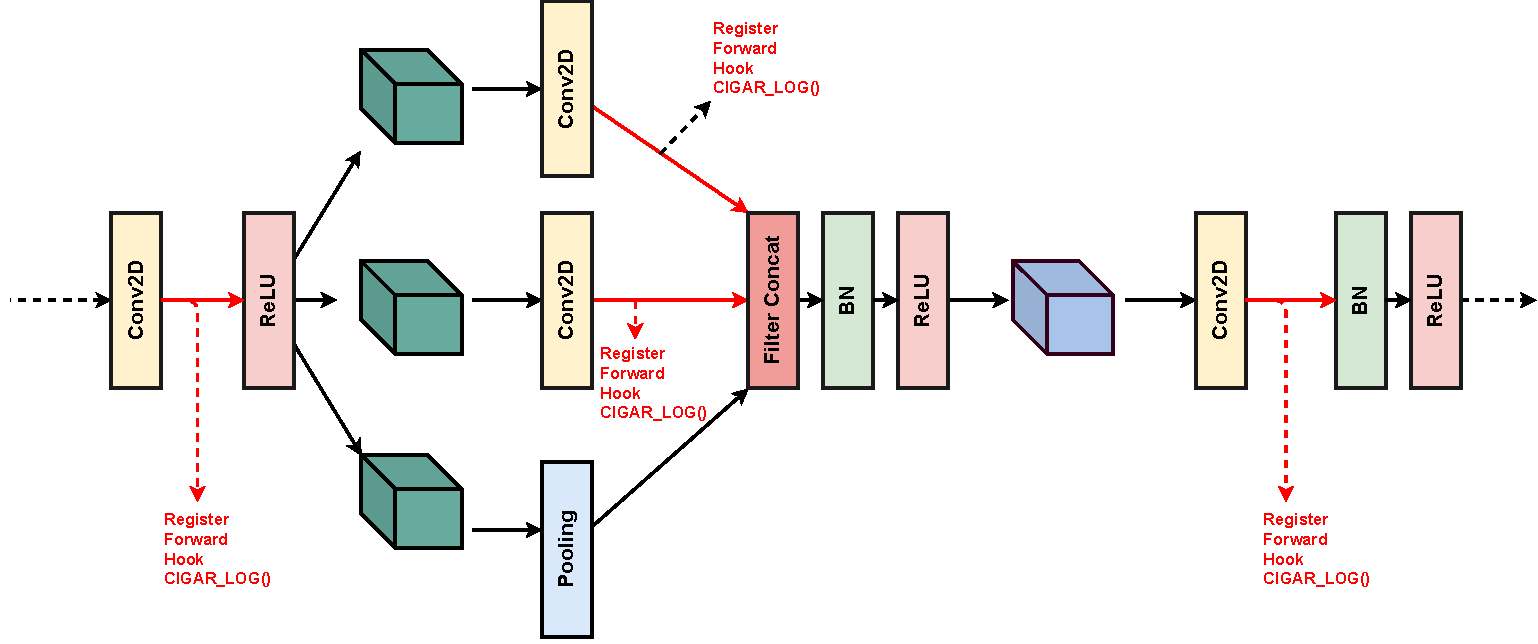
\includegraphics[scale=0.5]{fig/CIGAR.pdf}
    \caption{\ac{CIGAR} attachment of forward hooks to all model convolution layers}
    \label{fig:cigar_extraction}
\end{figure}

After all forward hooks are attached to the model, a forward pass of the model
is performed. Model layer statistics are added to the $model^{stats}_{dict}$ and
the collector's internal layer statistics tracker is reset. The layer statistics
collected for convolution layers are 1) the kernel sizes 2) strides 3) any additional padding
4) the number of convolution groups 5) kernel dilation. For linear layers the input and output feature sizes are collected.
For both layer types, input feature map dimensions are collected. 
After processing all of the models in $model_{dict}$, a $model^{stats}_{dict}$ is
returned for further analysis used to derive the necessary library insights for
pruning the dataflow design space. An illustration of that process is available
in \autoref{fig:cigar_flow}. New layers can be analyzed by CIGAR provided that the
collector is updated to be able to collect statistics from different layer types
and Attach\_Collection\_Hooks is allowed to attach the collector's callback
function to the newly supported layer. 

\begin{figure}
    \centering
    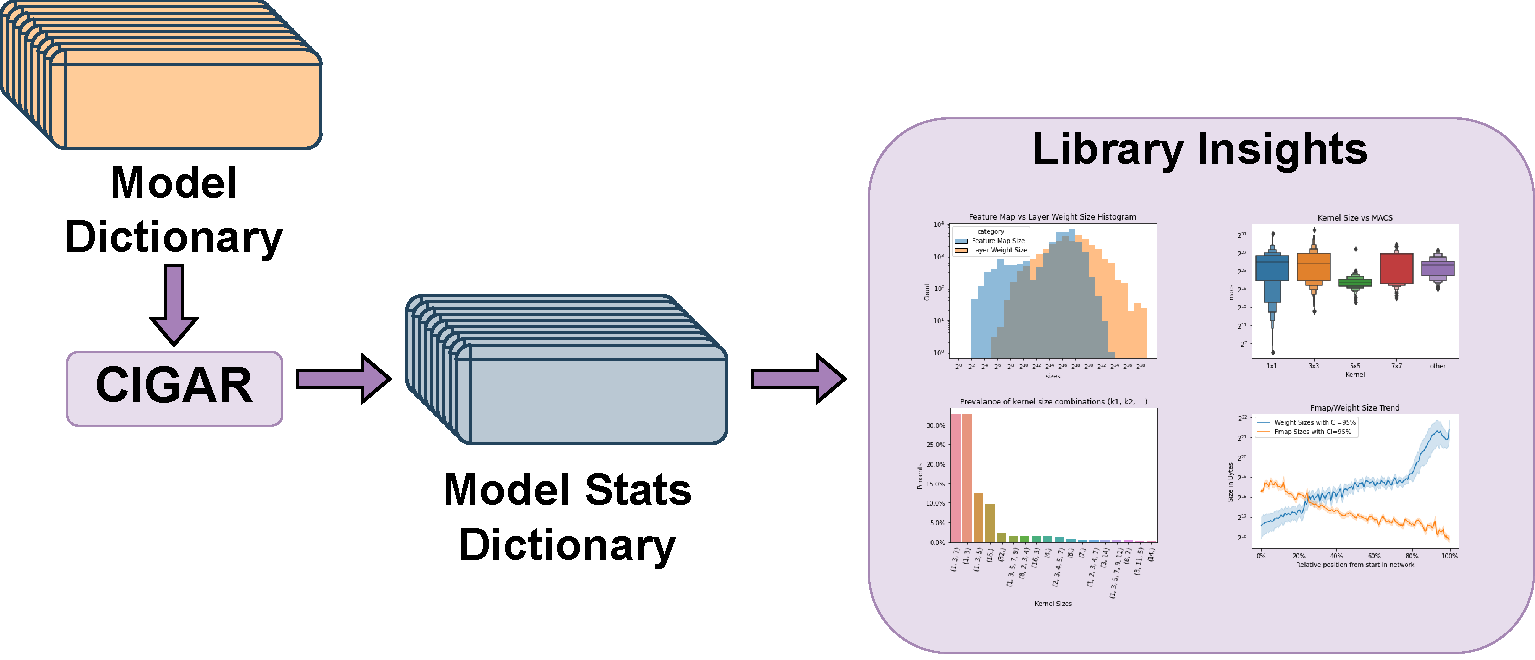
\includegraphics[scale=0.4]{fig/Cigar_flow.pdf}
    \caption{\ac{CIGAR} extraction of convolution layers}
    \label{fig:cigar_flow}
\end{figure}

\begin{algorithm}[H] 
    \caption{\ac{CIGAR}}
    \label{alg:cigar_algo}
    \begin{algorithmic}[1]
    \Require{$model_{dict}$} 
    \Ensure{$model^{stats}_{dict}$}
    \Statex
    \Function{Attach\_Collection\_Hooks}{$model, collector$}
        \State $hooks \gets []$
        \For{$layer \in model.named\_modules()$}
            \If{$type(layer)$ is $conv2d$ or $type(layer)$ is $linear$} 
                \State $hooks.push(layer.register\_forward\_hook(collector.layer\_collector))$
            \EndIf 
        \EndFor
    \State \Return{$hooks$}    
    \EndFunction
    \Statex
    \Function{Collect\_Library\_Statistics}{$model_{dict}$}
        \State $model^{stats}_{dict} \gets \{\}$
        \State $collector \gets Collector()$
        \For{$(model_{name}, model) \in model_{dict}$}
            \State $input\_img\_tensor \gets transform(open('default.jpg'), model)$
            \State $hooks \gets Attach\_Collection\_Hooks(model, collector)$
            \State $model.forward(input)$
            \State $model^{stats}_{dict}[model_{name}] \gets collector.model\_stats()$
            \State $collector.reset()$
            \State $hooks \gets Detach\_Collection\_Hooks(hooks)$
        \EndFor
        \State \Return {$model^{stats}_{dict}$}
    \EndFunction
    \end{algorithmic}
\end{algorithm}

\subsection{Neural Network Library Explored}
\label{chap:dda:dataflow_dse:pruning:cigar:library}

A diverse range of networks were explored by CIGAR for dataflow design space
pruning. The diversity of networks is reflected in the diversity of model types,
layer types, model sizes, and the number of MACs in the network. An illustration
of the model sizes vs number of MAC diversity is presented in
\autoref{fig:cigar_library_overview}. From \autoref{fig:cigar_library_overview}
it is clear that a wide range of models were selected as part of the CIGAR
library explored. The library includes smaller models like squeezenet and
mobilenetv2 as well as larger models like VGG16 \cite{dnn_is_sota_image}.
In terms of layer diversity the library includes conventional networks with both
convolution layers and linear layers as well as newer more exotic networks that
combine transformer self attention layers with convolution layers like CoAtNet
\cite{xu_co-scale_2021}. An illustration of that layer type diversity is
reflected in figure \autoref{fig:cigar_library_overview}.b. A total of 695 networks where explored.
The full list of networks explored is available in the
appendix of this thesis. All models explored by CIGAR were implemented in
pytorch and provided by either torchhub in \cite{pytorch} or the PyTorch Image
Models (timm) package in \cite{timm}.  

\begin{figure}
    \centering
    \subfigure[]{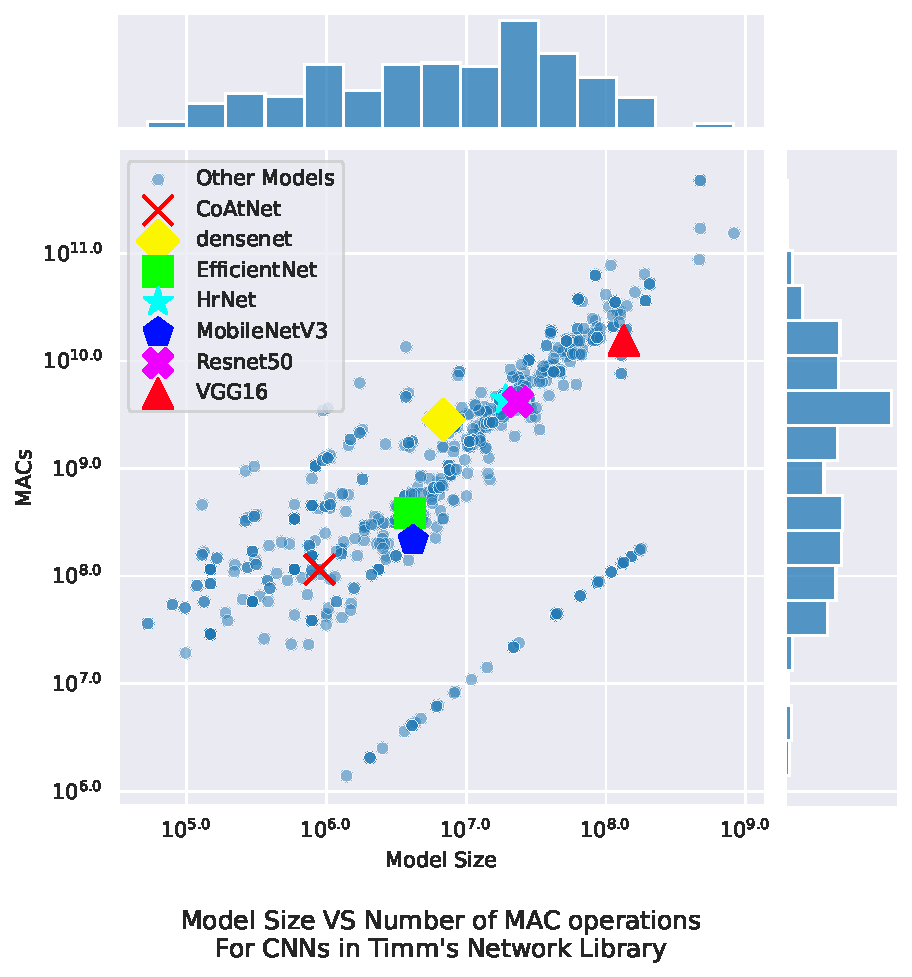
\includegraphics[width=0.495\textwidth]{Plots/overview/macs_vs_size.pdf}}
    \subfigure[]{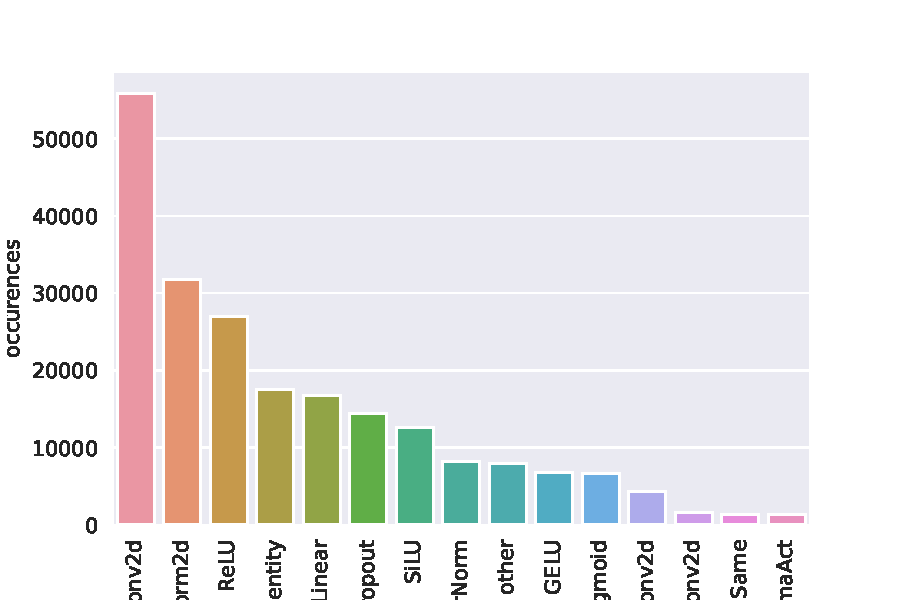
\includegraphics[width=0.495\textwidth]{Plots/overview/layer_types.pdf}}
    \caption{Illustration of CIGAR's library diversity based on (a) Model sizes and number of MACS (b) Model layer types}
    \label{fig:cigar_library_overview}
\end{figure}

\clearpage

\subsection{Pruning the Dataflow Design Space using CIGAR}
\label{chap:dda:dataflow_dse:pruning:applying_it}

Using CIGAR, the process of pruning the dataflow design space can begin. As
mehtioned earlier from \cite{dnn_df_overrated}, the available dataflow design
space dimensions of the convolution operation are (1) unroll targets (2) loop
unroll factors (3) spatial axis mapping. We can prune the design space partially by
identifying loop unroll targets as well as loop unroll factors for the kernel
loops of the dataflow. This partial pruning will enable the reuse
analysis presented in \autoref{chap:dda:hw_dse} necessary for the application of the hardware implementation taxonomy
provided by \cite{maestro}.

\subsubsection{Loop Unroll Targets}
\label{chap:dda:dataflow_dse:pruning:applying_it:loop_unroll_targets}

The choice of loop unroll targets affects the stationarity of the data elements
in the convolution operation within compute elements of a Convolution
accelerator. For example, assuming a convolution layer with a
kernel size of (2, 2), if we unroll the F, C, KY, KX loops by a factor of 2,
weight element batches of size 16 will be loaded on to the chip in order to
compute the output feature map. These weight will remain stationary until all
input featuremap elements are loaded and consumed to evaluate the relevant
partial sums associated with the filter weights loaded. In this scenario, the
stationarity of the weight elements exceeds that of the input featuremap and
output featuremap elements.   


We can determine what loop targets should be unrolled based on the
stationarity of each date type present in the convolution operation. A data
element that exhibits a high degree of stationarity should remain on chip for as
long as possible in order to minimize excessive reloads from off chip memory. We
can use the number of MAC operations a data element participates in as a
surrogate for stationarity. A data elements element reused across many MAC operations
should be kept on chip for as long as possible to avoid excessive reloading of
that element from of-chip dram. Using CIGAR we can analyze data element reuse
behavior in all models of the TIMM library for the three data elements present in the convolution operation, input
feature maps elements (IFmaps), output feature map elements (OFmaps), and weight
elements. The results from this analysis are present in
\autoref{fig:reuse_behavior}. 

\begin{figure}
    \centering
    \subfigure[]{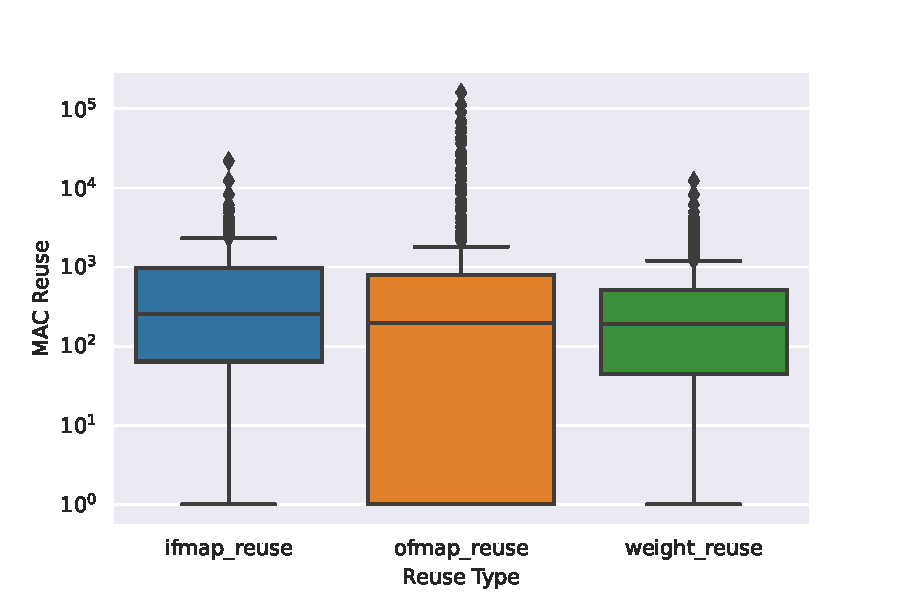
\includegraphics[width=0.495\textwidth]{Plots/reuse/reuse_box.pdf}}
    \subfigure[]{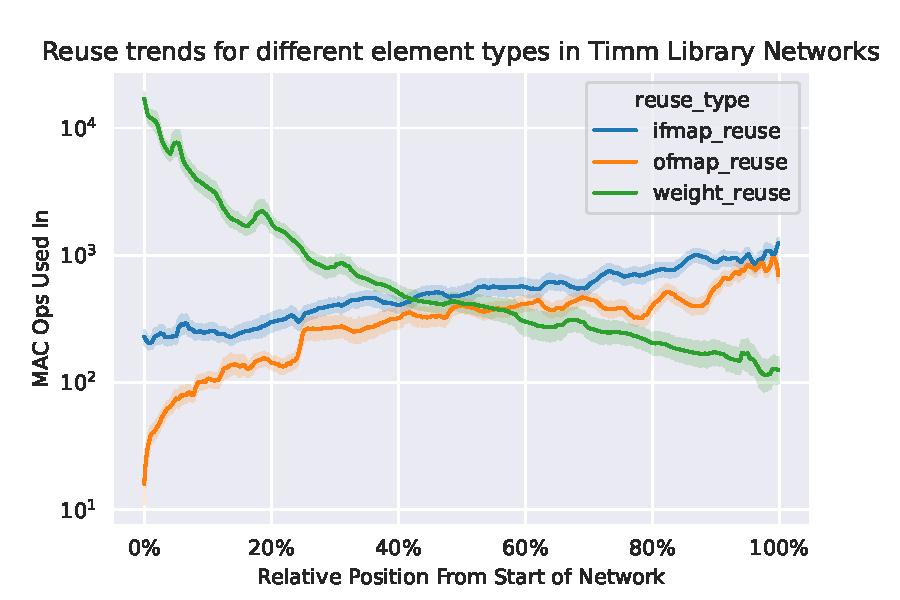
\includegraphics[width=0.495\textwidth]{Plots/reuse/reuse_trends.pdf}}
    \caption{Exploration of data element reuse behavior in convolution layers of models from the TIMM library, a) shows overall reuse behavior as a boxplot b) shows reuse behavior trends within models with multiple convolution layers}
    \label{fig:reuse_behavior}
\end{figure}


From \autoref{fig:reuse_behavior}.a the reuse behavior between all three data
elements is comparable with the exception OFmap reuse having a much lower 0.25
quantile. IFmap elements have a slightly higher reuse with the median MAC
operations performed per element load equal to 256 MACs. Weight and OFmap
elements exhibit lower reuse at 192 and 196 MACs per load. Reuse trends within
networks show a general shift from high weight reuse to high IFmap and OFmap
reuse depending on the relative position from start within a network. Weight
reuse is initially almost 2 orders of magnitude higher than IFmap and OFmap
reuse, however, since the shift in reuse behavior happens relatively early in
most networks, higher IFmap reuse exceeding weight and OFmap reuse persists for
more layers within an network. These findings indicate that all elements can
benefit from stationarity depending on the network and even the layer position
within a network. For an accelerator with a fixed dataflow the choice of
dataflow and hence which loops to unroll is heavily influenced by the target
networks expected to run on the accelerator. The most appropriate dataflow in this
case is weight stationary dataflow which takes advantage of the comparatively higher weight
reuse in the earlier layers of most networks by keeping weights stationary
within the compute elements of HERO. Weight stationary arises from choosing the F, C, KY and KX loops are the
unroll targets. Additionally, the overlap between weight stationary under (1, 1)
convolutions and GEMM (discussed in 
\autoref{chap:dda:dataflow_dse:GEMM_mode:conv_gemm_equiv:proof}) enables support for arbitrary convolution and
linear layers via transformation in \cite{cafe_con_troll}.

% The choice
% of a weight stationary dataflow lends itself well to \ac{GEMM} given the
% similarities in the loop structure with regards to F and C loops for both
% applications. Furthermore, a weight stationary based dataflow allows support for
% linear layers through this overlap which are quite prevalent in many modern
% networks as seen in \autoref{fig:cigar_library_overview}.b. Given the
% flexibility of weight stationary, F, C, KY and KX loops will be the loop unroll
% targets. 

This choice of dataflow effectively creates two operational modes. A direct mode
where convolution operations with kernels that are supported directly are
executed on the accelerator and a GEMM mode where kernels that are not supported
directly are supported by a data transformation technique from
\cite{cafe_con_troll} followed by conversion of the proceeding GEMM operation
into a (1, 1) convolution. A full explanation of GEMM mode is given in
\autoref{chap:dda:dataflow_dse:GEMM_mode}. 

Note that convolution layers with non (1, 1) strides are executed under GEMM
mode. Supporting convolution layers with non (1, 1) strides directly is left as
part of future work. From \autoref{fig:kernel_stats:strides} (1, 1) strides are
present in ~95\% of convolution layers so the implications of indirect support
of non (1, 1) strides via GEMM mode will likely be negligible when assessing the overall
performance and energy efficiency of an accelerator implementing the
aforementioned operation modes.

% \clearpage
\begin{figure}
    \centering
    \subfigure[]{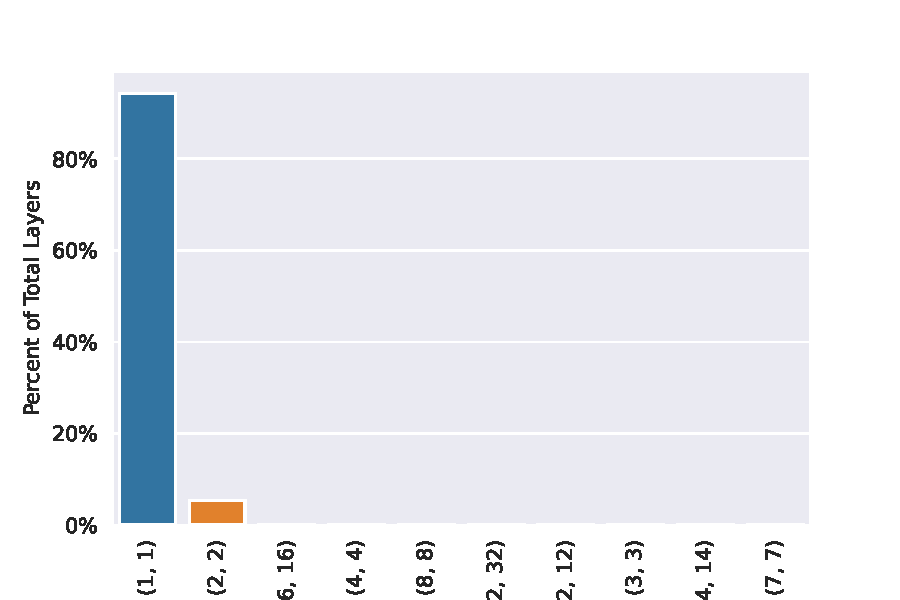
\includegraphics[width=0.495\textwidth]{Plots/kernel/strides.pdf}}
    \caption{Percentage of total layers in the TIMM library's networks that have a stride size (k, k)}
    \label{fig:kernel_stats:strides}
\end{figure}


% \clearpage
% \begin{lstlisting}[language=C, caption=Weight stationary dataflow, label={lst:conv_loop}]
% #pragma UNROLL F_UNROLL
% for(int f = 0; f < F; f+=F_UNROLL) // Filter loop
% #pragma UNROLL C_UNROLL
%     for(int c = 0; c < C; c+=C_UNROLL) // Channel loop
%         for(int y = 0; y < Y; y+=1) // Output feature map row
%             for(int x = 0; x < X; x+=1)  // Output feature map col
% #pragma UNROLL KY_UNROLL
%                 for(int ky = 0; ky < KY; ky+=KY_UNROLL)  // Kernel row
% #pragma UNROLL KX_UNROLL
%                     for(int kx = 0; kx < KX; kx+=KX_UNROLL)  // Kernel col
%                         O[f][y][x] += I[c][y+ky][x+kx]*W[f][c][ky][kx];
% \end{lstlisting}

% \begin{lstlisting}[language=C, caption=GEMM loops, label={lst:W_S_Generic_Loop}]
%     #pragma unroll F_UNROLL
%     for(int f = 0; f < F; f+=F_UNROLL) // Filter loop
%     #pragma unroll C_UNROLL
%         for(int c = 0; c < C; c+=C_UNROLL) // Channel loop
%             for(int z = 0; z < Z; z+=1)
%                 O[f][z] += W[f][z]*I[c][z];
% \end{lstlisting}

\subsubsection{Loop Unroll Factors}
\label{chap:dda:dataflow_dse:pruning:applying_it:loop_unroll_factors}

There exists significant variation with regards to the kernel sizes present in
the TIMM library. This makes the question of unroll factors and axis mapping for
the KY and KX loops more difficult to answer.

From \autoref{fig:kernel_stats:freq}.a (1, 1) and (3, 3) kernel sizes dominate in
comparison to all other kernel sizes. This renders the choice of keeping KY and
KX loops folded impractical because if support is extended to an arbitrary K x K
kernel while keeping KY and KX loops are folded, the onboard storage for weights would
then need to be at least $K^2$ where $K$ is the upper bound of kernels supported
directly to avoid excessive weight fetches from DRAM. Unfortunately, for ~80\% of
the layers in the network, that additional storage area would be significantly
underutilized by a factor of $\frac{1}{K^2}$ due to the overrepresentation of
1x1 kernels. To mitigate this under utilization of onboard memory for weights, KY
and KX loops need to be unrolled fully. However, this begs the question, what
kernel sizes should be assumed when unrolling the KY and KX loops? Any kernel
sizes assumed when unrolling KY and KX loops become kernel sizes that are
supported directly. Kernel sizes that are not assumed when unrolling KY and KX
loops can be supported via GEMM mode. This means that (1, 1)
kernels are supported directly by necessity since they are what enable GEMM mode
to begin with. Other kernel sizes to support directly can be derived from
\autoref{fig:kernel_stats:freq}. In \autoref{fig:kernel_stats:freq}.b many
networks contain at least 1 convolution layer that is not (1, 1) or (3, 3). For
example a (7, 7) kernel exists in around ~20\% of networks. The reason for the
prevalence of (7, 7) convolutions originates from the historical use of resnet
\cite{resnet} as a feature extractor for a significant portion of networks
analyzed by CIGAR.

\begin{figure}
    \centering
    \subfigure[]{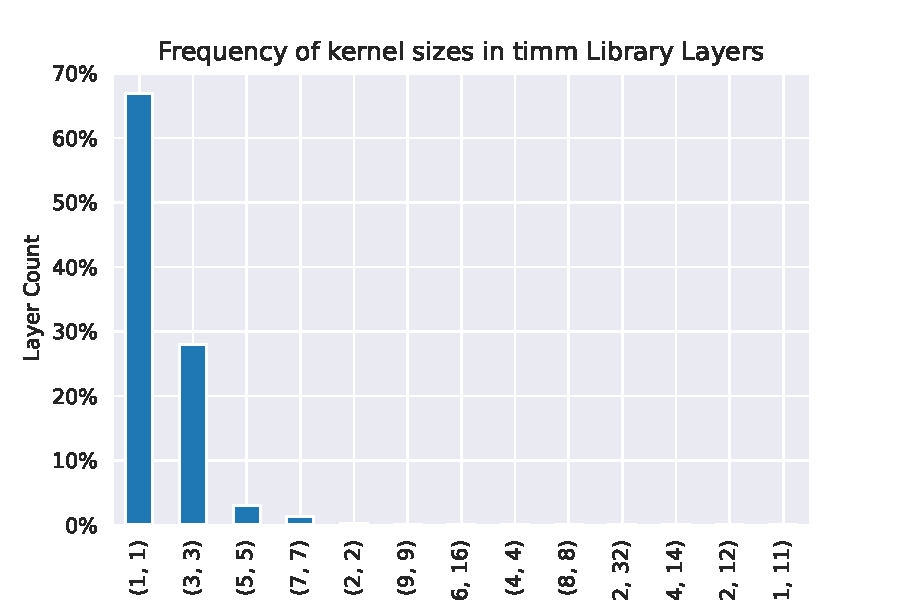
\includegraphics[width=0.495\textwidth]{Plots/kernel/freq.pdf}}
    \subfigure[]{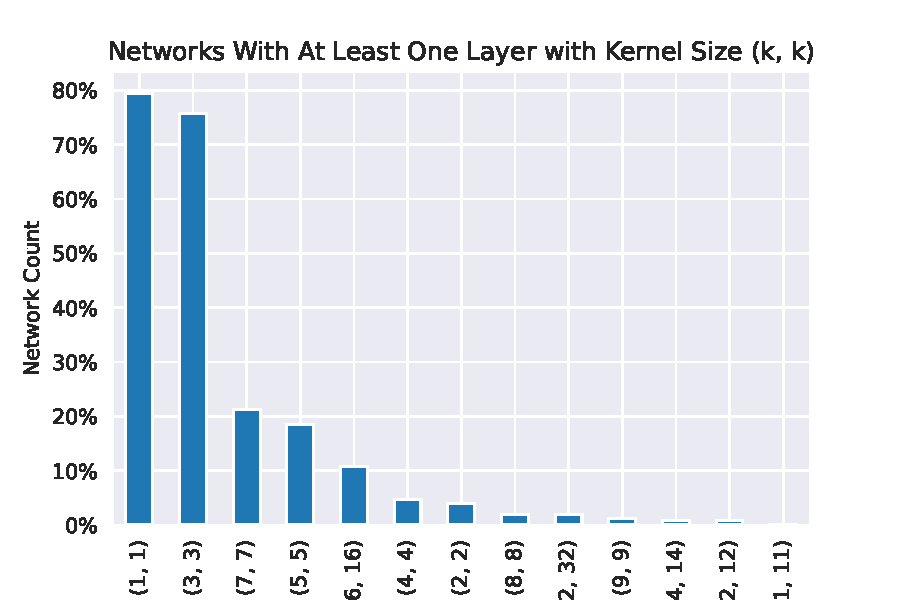
\includegraphics[width=0.495\textwidth]{Plots/kernel/at_least.pdf}}
    \caption{(a) Percentage of total layers in the TIMM library's networks that have a kernel size (k, k) (b) The percentage of networks in TIMM that have at least one kernel of size (k, k)}
    \label{fig:kernel_stats:freq}
\end{figure}


In \autoref{fig:kernel_vs_mac}.a, when adjusting for the the number of MACs
present in layers where these kernel sizes exist, (1, 1) and (3, 3) kernels share a
similar computational burden on the network with (1, 1) having a much wider spread.
7x7 kernels have a much tighter spread but they still represent a similar
computational burden to (1, 1) and (3, 3) kernels in networks where they are present.
Adjusting for kernel frequency in \autoref{fig:kernel_vs_mac}.b, (1, 1) and (3, 3)
kernels dominate all other kernel sizes in terms of number of MACs in most
network layers. From \autoref{fig:kernel_vs_mac} it is clear that (1, 1) and (3, 3)
kernels need to be supported directly while all other kernels need to be
supported via GEMM mode. 

This limits the space of possible unroll
factors for the loop unroll targets and thus prunes the dataflow design space.
Supporting kernels via GEMM mode lead to an expansion of the IFmap due to the
duplication introduced by lowering, however that expansions is negligible given
the relative infrequency of non (1, 1) and (3, 3) layers. 

% What remains of the dataflow
% design space under weight stationary is 1) the unroll factors for F and C loops
% and 2) the axis mapping for F, C, KY and KX loops for the 2 spatial axis of a
% convolution accelerator. However, since the design space has been partially
% pruned by selection the loop unroll targets and the loop unroll factors for the
% kernel loops, an analysis of reuse is possible via the approach in \cite{meeus}. 

% To explore the what remains of the dataflow design
% space an automated dataflow exploration tool will be introduced and discussed in
% \autoref{chap:arch_dimensioning}.   

\begin{figure}
    % Todo: update figure titles to reflect origins of statistics
    \centering
    \subfigure[]{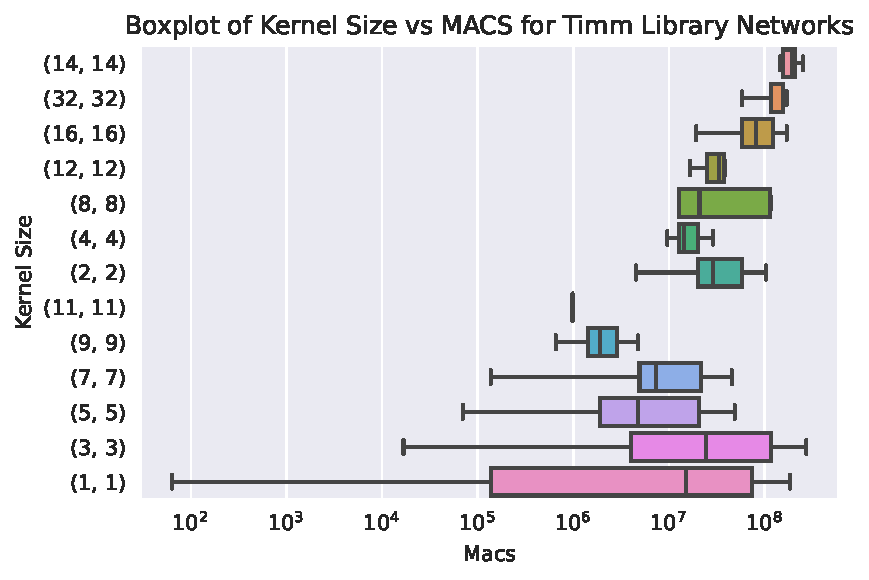
\includegraphics[width=0.495\textwidth]{Plots/kernel/macs.pdf}}
    \subfigure[]{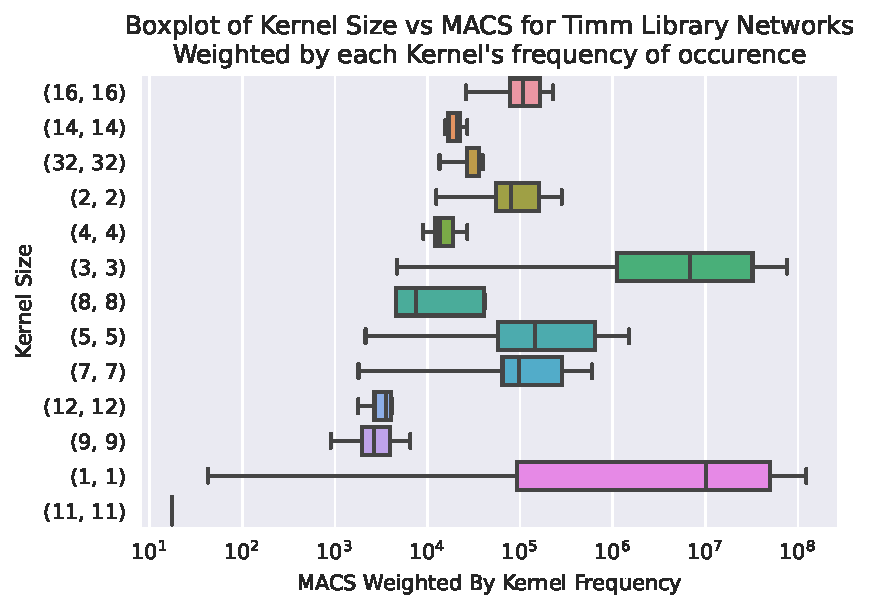
\includegraphics[width=0.495\textwidth]{Plots/kernel/macs_adjusted.pdf}}
    \caption{(a) Kernel size vs number of layer MACs  (b) Kernel size vs number of layer MACs adjusted by kernel frequency}
    \label{fig:kernel_vs_mac}
\end{figure}

% % TODO: Introduce tiling discussion here using tiling figure

\subsection{A note on accelerator Spatial Axis mapping}
\label{chap:dda:dataflow_dse:GEMM_mode:axis_mapping}

While determining spatial axis mapping is part of the second part of pruning of the
dataflow design space, spatial axis mapping has implications regarding the
effective unroll factors for the F and C loops when the share the same spatial
axis as the unrolled kernel loops. These implications are discussed in this
subsection. 

When determining axis mapping, F and C loops are assumed to be bound to an
accelerator's vertical and horizontal spatial axis. Utilizing both axis results
in better overall on-chip area utilization assuming conventional 2 dimensional
constraints for chip fabrication. Mapping all loops to the same axis can provide
the most flexibility with regards to the allocation of PEs as a resource to
process different filters, channels and kernels. However, this complicates on
chip connectivity. KY and KX loops can then be
bound to either the horizontal or vertical axis of an accelerator based on the
variable $K_{axis}$.  Depending on which axis KY and KX loops are mapped, the
effective unroll factors for F and C loops ($F_{eff}$ and $C_{eff}$) are
changed. If the unrolled kernel loops share the same axis as the C loops, the
effective $C_{unroll}$ factor for the C loops is then $\lfloor
\frac{C_{unroll}}{K_{unroll}} \rfloor$ which means the effective C unroll factor
decreases depending on the size of the kernel unroll factor. This decrease in
effective unroll factor arises from the fact that, within the same axis as the C
loops, compute resources are allocated to process a single $K^2_{unroll}$ kernel. This
results in a decrease of compute resources available to process other channels
concurrently. The same logic applies to F loops if the Kernel loops are mapped
to the same axis vertical axis as they are. This idea is presented in
\autoref{math:effective_unroll_factors_c} and
\autoref{math:effective_unroll_factors_f}. In both equations $F_{unroll}$ and
$C_{unroll}$ are the unroll factors for F and C loops assuming $KY=KX=K=1$.


\begin{align}
    \begin{gathered}
        C_{eff} = \begin{cases} \lfloor \frac{C_{unroll}}{K^{2}_{unroll}} \rfloor & K_{axis} = horizontal\\ C_{unroll} & K_{axis} = Vertical\end{cases} \\
        \end{gathered}
    \label{math:effective_unroll_factors_c}
\end{align}
\begin{align}
    \begin{gathered}
        F_{eff} = \begin{cases} \lfloor \frac{F_{unroll}}{K^{2}_{unroll}} \rfloor & K_{axis} = Vertical\\ F_{unroll} & K_{axis} = Horizontal\end{cases} \\
        \end{gathered}
    \label{math:effective_unroll_factors_f}
\end{align}


In summary, by selecting weight stationary as the chosen dataflow for HERO we
can 1) take advantage of the high weight reuse observed in
many networks and 2) extend support
to arbitrary convolution/ linear layers via GEMM mode which arises by
reinterpreting (1, 1) convolution as GEMM operations. Weight stationary sets the
loop unroll targets to the F, C, KY, and KC loops, with the assumption that the
stride size is limited to (1, 1) due to its substantial prevalence. By unrolling the F, C
loops we can maximize weight reuse as well as parallelize layers that have been
converted to GEMM.

Keeping KY and KX loops folded is impractical with respect to efficient on-chip
memory utilization because the vast majority of convolution layers have (1, 1)
kernel sizes. By considering the frequency of occurrence and the number of MACs,
we choose to unroll the KY and KX loops to (3, 3). Additionally, since (1, 1)
kernel sizes form the basis of GEMM mode which strengthens the argument for
direct support (1, 1) kernels.

The next section examines the theoretical underpinnings of the overlap between
(1, 1) convolutions and GEMM and how support can be extended to arbitrary
convolutions through this overlap when used in tandem with data transformation
approaches from \cite{cafe_con_troll}.

% The unroll factor for F and C loops remains open, and will be further explored
% in a later chapter of this thesis using TEMPO. The act of unrolling these loops
% effectively tiles the weight tensor, allowing HERO to process a layer as a
% sequence of weight tiles. This raises the question of weight tile scheduling,
% which will be discussed in \autoref{chap:net_compile}.

\clearpage 

\section{Increasing Generality of a Direct Convolution Accelerator}
\label{chap:dda:dataflow_dse:GEMM_mode}

GEMM mode allows HERO to support arbitrary convolution operations by first
interpreting them as GEMM operations via one of the data transformation
approaches outlined in \cite{cafe_con_troll} then reinterpreting them as (1, 1)
convolutions which, from the previous section, are one of the kernel sizes
directly supported by HERO. This section discussess the overlap between GEMM and
(1, 1) convolutions which forms the bases of GEMM mode in HERO. 

Convolution operations can be converted into general matrix multiplication
through the use of lowering and lifting techniques like Im2col discussed in
\cite{cafe_con_troll}. This approach
to supporting arbitrary convolution operations would still require a matrix
multiplication accelerator. To support matrix multiplication within a
convolution accelerator we can either:

1) Repurpose existing compute and memory hardware on chip to perform both GEMM
and convolutions operations 

2) Establish a mathematical equivalence between GEMM operations and Conv
operations by reinterpret GEMM into a special case of convolution, namely
convolutions with a (1, 1) kernel size. 

This avoids the overhead of repurposing existing convolution hardware to support
GEMM. Once this relationship between GEMM and (1, 1) Convolutions is defined,
layers that are unsupported directly can be converted into equivalent layers
that are supported directly. In
\autoref{chap:dda:dataflow_dse:GEMM_mode:conv_gemm_equiv:proof}, a proof for the
equivalence between GEMM and (1, 1) Convolutions is given. Additionally, in
\autoref{chap:dda:dataflow_dse:GEMM_mode:layer_equivelence} the aforementioned
proof will be used in tandem with the approach in \cite{cafe_con_troll} to
provide support for arbitrary convolution operations. Finally, a discussion of
layer dimensionality for unsupported layers that have been converted to
equivalent supported layers is given in
\autoref{chap:dda:dataflow_dse:GEMM_mode:layer_dimentionality}.  

\clearpage

\subsection{Functional equivalence between GEMM and (1, 1) Convolutions}
\label{chap:dda:dataflow_dse:GEMM_mode:conv_gemm_equiv:proof}

We can establish the functional equivalence between GEMM and (1, 1) convolutions with
the following proof. An illustration of this proof is given in
\autoref{fig:gemmTo1x1Conv}.  
Given two matrices $A\in \mathbb{R}^{Z \times C}$ and $B \in \mathbb{R}^{C
\times F}$, let $R \in \mathbb{R}^{Z\times F} = A.B$. A different way to express
the matrix multiplication $A.B$ is \autoref{math:gemm_array_notation}.  

\begin{equation}
    \begin{aligned}
        R[z][f] = \displaystyle\sum\limits_{c=0}^{C-1}A[z][c]\times B[c][f] \\ \forall z\in[0, n^2-1]
    \end{aligned}
    \label{math:gemm_array_notation}
\end{equation}

Transposing $A$ and $B$ yields $\hat{A} \in \mathbb{R}^{C\times Z}$ and $\hat{B} \in
\mathbb{R}^{F\times C}$. Using the identity $(A.B)^T = B^T.A^T$ we can rewrite
\autoref{math:gemm_array_notation} as
\autoref{math:gemm_array_notation_transpose} where $\hat{R} \in
\mathbb{R}^{F\times Z}$

\begin{equation}
    \begin{aligned}
        \hat{R}[f][z] = \displaystyle\sum\limits_{c=0}^{C-1}\hat{B}[f][c]\times \hat{A}[c][z] \\ \forall z\in[0, Z-1]
    \end{aligned}
    \label{math:gemm_array_notation_transpose}
\end{equation}

We can reshape $\hat{A}$ and $\hat{B}$ using \autoref{math:a_b_reshape} into 3D
tensors by adding an additional dimension of size 1 for $\hat{A}$ and 2
additional dimensions of size 1 for $\hat{B}$.

\begin{equation}
    \begin{aligned}
        \hat{A} \xrightarrow[]{Reshape} &\hat{A}  \in \mathbb{R}^{C \times Z\times 1}   &\hat{B} & \xrightarrow[]{Reshape} \hat{B}  \in \mathbb{R}^{F \times C\times 1\times 1} \\
    \end{aligned}
    \label{math:a_b_reshape}
\end{equation}

Applying \autoref{math:a_b_reshape} to
\autoref{math:gemm_array_notation_transpose} yields
\autoref{math:gemm_as_conv_1} where $\hat{R} \in \mathbb{R}^{F \times Z\times 1}
$ remains the transposed output of $A.B$. 

\begin{equation}
    \begin{aligned}
        \hat{R}[f][z][0] = \displaystyle\sum\limits_{c=0}^{C-1}\hat{A}[c][z][0]*\hat{B}[f][c][0][0] \\ \forall z \in [0, Z-1] 
        \end{aligned}
    \label{math:gemm_as_conv_1}
\end{equation}

Adding kernel summations to \autoref{math:gemm_as_conv_1} yields
\autoref{math:gemm_as_conv_2} which is equivalent to a (1, 1) convolution of stride
1. To recover $R$ from $\hat{R}$ we can reshape $\hat{R}$ by removing the
last dimension and then transpose it. 

\begin{equation}
    \begin{aligned}
        \hat{R}[f][z][0] = \displaystyle\sum\limits_{c=0}^{C-1}\displaystyle\sum\limits_{k_x=0}^{1} \displaystyle\sum\limits_{k_y=0}^{1}\hat{A}[c][y+ky][x+kx]*\hat{B}[f][c][k_y][k_x] \\ \forall y \in [0, Z-1] \land x = 0
    \end{aligned}
    \label{math:gemm_as_conv_2}
\end{equation}

\begin{figure}[]
    \centering
    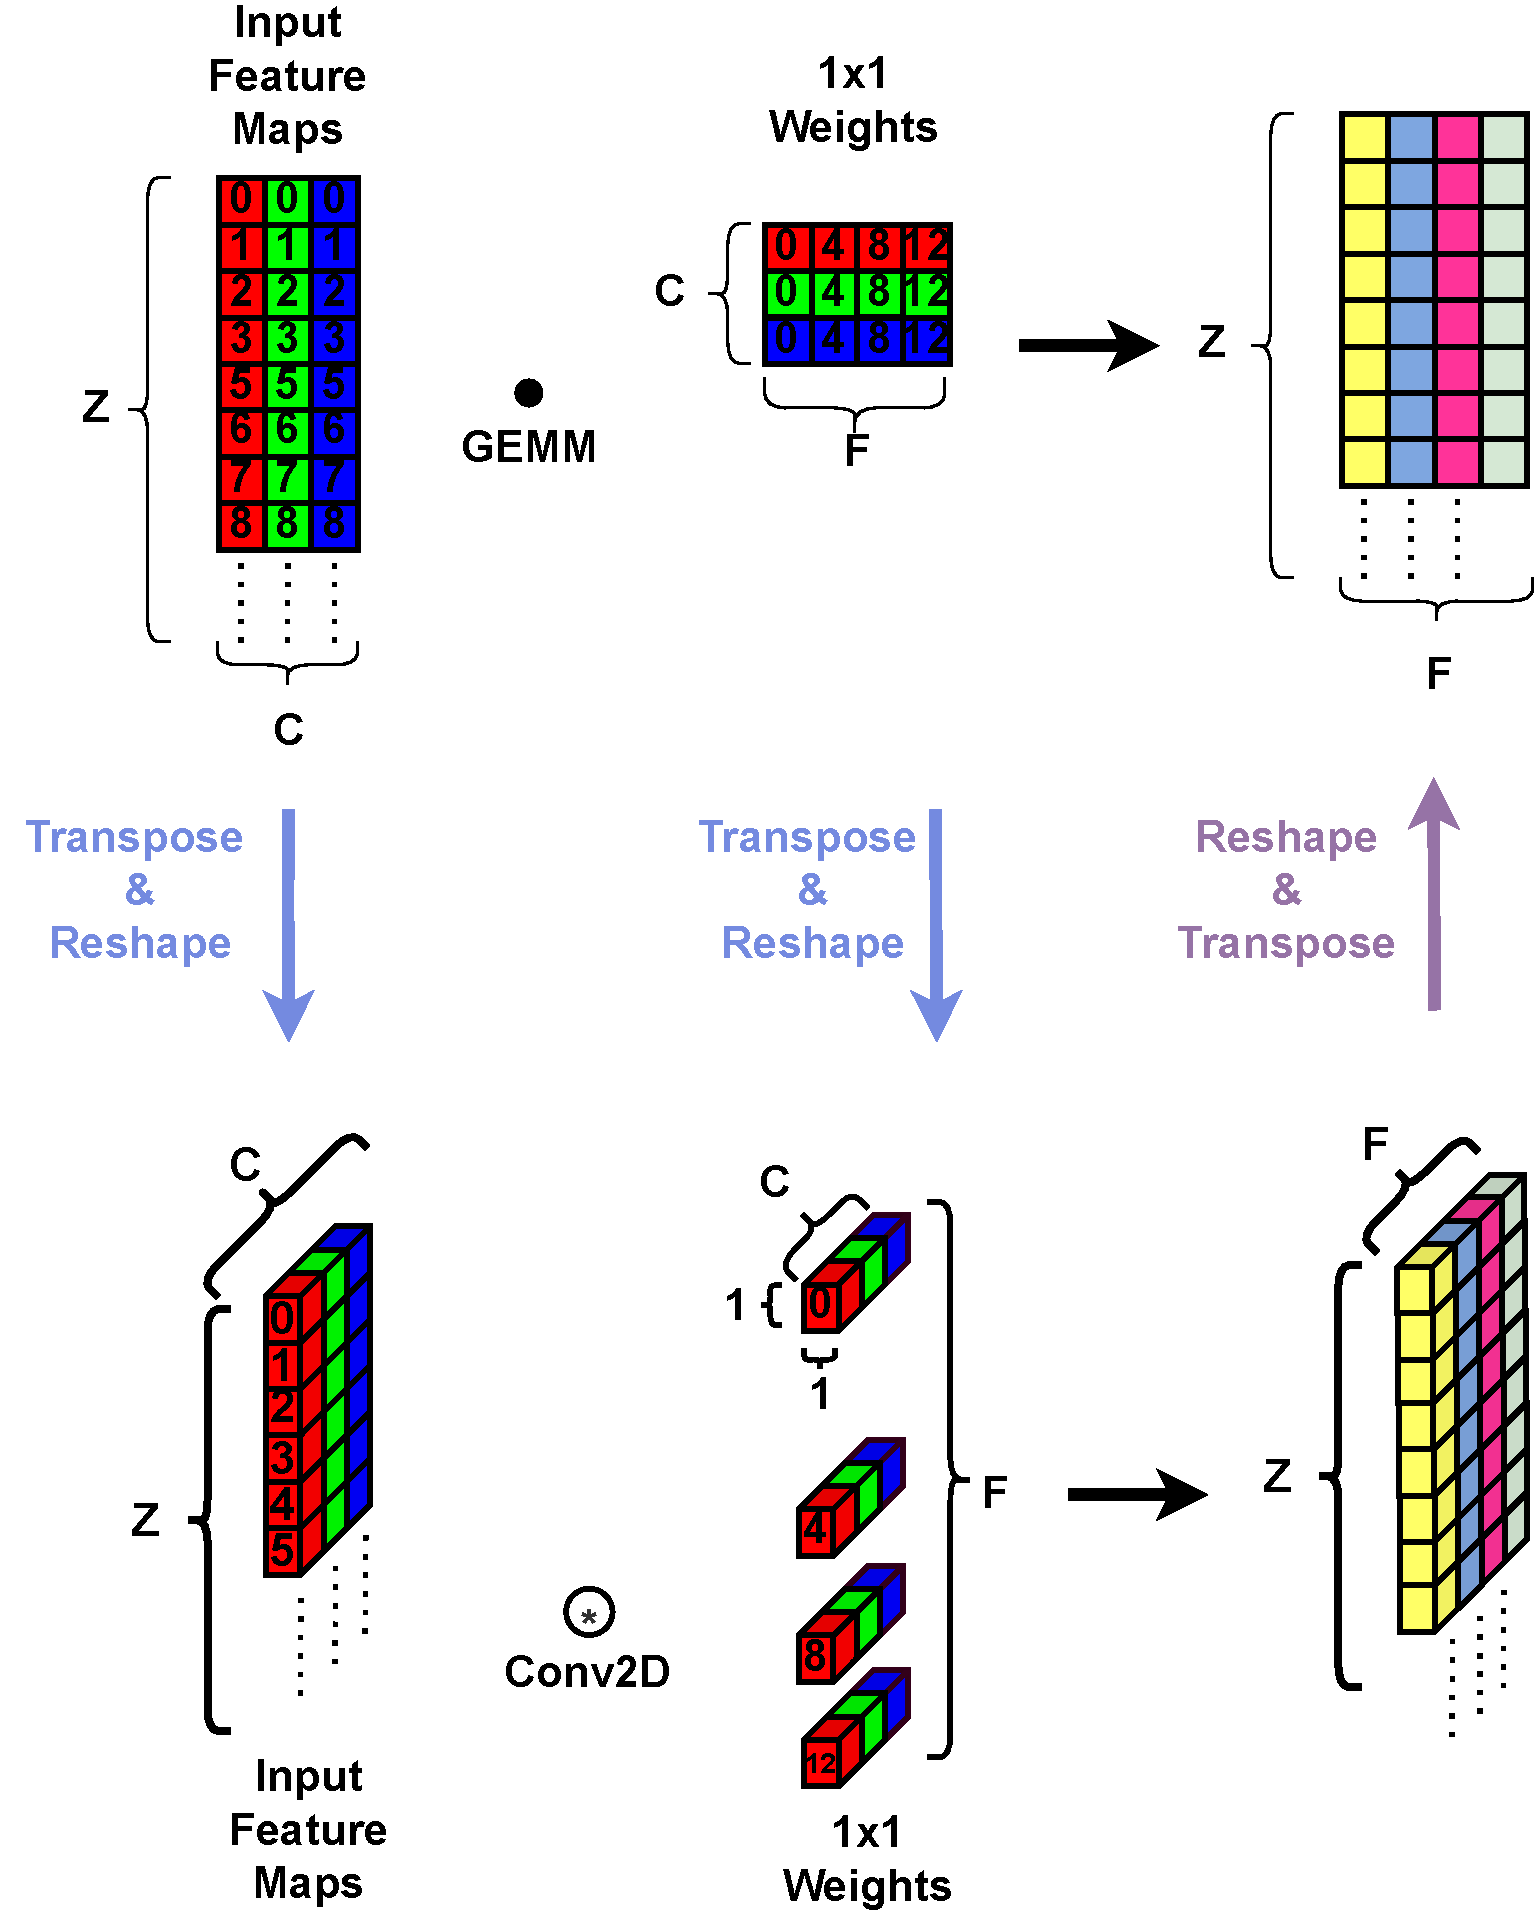
\includegraphics[scale=0.5]{fig/GemmTo1x1Conv.pdf}
    \caption{\ac{GEMM} and (1, 1) Convolution Equivalence}
    \label{fig:gemmTo1x1Conv}
\end{figure}


\subsection{Layer Equivalence}
\label{chap:dda:dataflow_dse:GEMM_mode:layer_equivelence}

We can support previously unsupported kernel sizes by combining the GEMM to (1, 1)
Conv conversion in
\autoref{chap:dda:dataflow_dse:GEMM_mode:conv_gemm_equiv:proof} with any
tensor lowering/lifting approach in \cite{cafe_con_troll}. Lowering converts a
convolution into a GEMM operation, and the approach in
\autoref{chap:dda:dataflow_dse:GEMM_mode:conv_gemm_equiv:proof} reinterprets
that operation as another (1, 1) Convolution. This approach allows any convolution
accelerator that can support (1, 1) convolution operations with asymmetric IFmaps
to support any arbitrary convolution operation. A visual illustration for this
technique is presented in \autoref{fig:conv2gemm2conv}. To demonstrate this
approach we begin by lowering both IFmap using
\autoref{math:balanced_lowering_ifmap} and Weights using
\autoref{math:balanced_lowering_weight}. This results in two matrices IFmap and
Weights in \autoref{math:conv2gemm2conv:lowering}. Lowering should be performed
if the kernel size of the Weight tensor is unsupported $K' \notin
\{SupportedKernels\}$. 

\begin{equation}
    \begin{aligned}
        IFmap \in R^{C\times n\times n} & \xrightarrow[]{Balanced Lowering} \hat{IFmap} \in R^{nm\times K'C} \\
        Weight \in R^{F\times C\times K' \times K'} & \xrightarrow[]{Balanced Lowering} \hat{Weight} \in R^{K'C\times K'F} \\
    \end{aligned}
    \label{math:conv2gemm2conv:lowering}
\end{equation}

After lowering both tensors, we apply the transformations in
\autoref{math:conv2gemm2conv:transform} to reinterpret the anticipated GEMM
operation that occurs after lowering into a (1, 1) convolution operation. The
transformations are composed of a transpose operation followed by a reshape
operation that appends additional dimensions of size 1 to both IFmap and
Weights. The transformations yields two new tensors $\hat{IFmap}$ and
$\hat{Weight}$.

\begin{equation}
    \begin{aligned}
        \hat{IFmap}^T \in R^{K'C \times nm} & \xrightarrow[]{Reshape} \hat{IFmap} \in R^{K'C \times nm \times 1} \\
        \hat{Weight}^T \in R^{K'F\times K'C} & \xrightarrow[]{Reshape} Weight \in R^{K'F\times K'C \times 1 \times 1} \\
        \end{aligned}
    \label{math:conv2gemm2conv:transform}
\end{equation}

After performing the transformations in \autoref{math:conv2gemm2conv:transform}
the output $\hat{OFmap_{prelift}}$ can be calculated after performing a (1, 1)
convolution in \autoref{math:conv2gemm2conv:conv} using the $\hat{IFmap}$ and
$\hat{Weight}$ tensors. 

\begin{equation}
    \begin{aligned}
        \hat{OFmap_{prelift}} \in R^{K'F\times nm \times 1} = \hat{IFmap}*\hat{Weight}
        \end{aligned}
    \label{math:conv2gemm2conv:conv}
\end{equation}

Finally we can lift $\hat{OFmap_{prelift}}$ by first reshaping it into a 2D
matrix by dropping the last dimension and then transposing it. After that, we
can apply balanced lifting in \autoref{math:balanced_lifting_ofmap} to get the
final OFmap in \autoref{math:conv2gemm2conv:lift}.

\begin{equation}
    \begin{aligned}
        \hat{OFmap_{prelift}} \in R^{K'F \times nm \times 1} \xrightarrow[]{Reshape} OFmap_{prelift} \in R^{K'F\times nm} \\
        OFmap_{prelift}^T \in R^{nm\times FK} \xrightarrow[]{Balanced Lifting} OFmap \in R^{F \times m \times m} \\
            \end{aligned}
    \label{math:conv2gemm2conv:lift}
\end{equation}

\begin{figure}[]
    \centering
    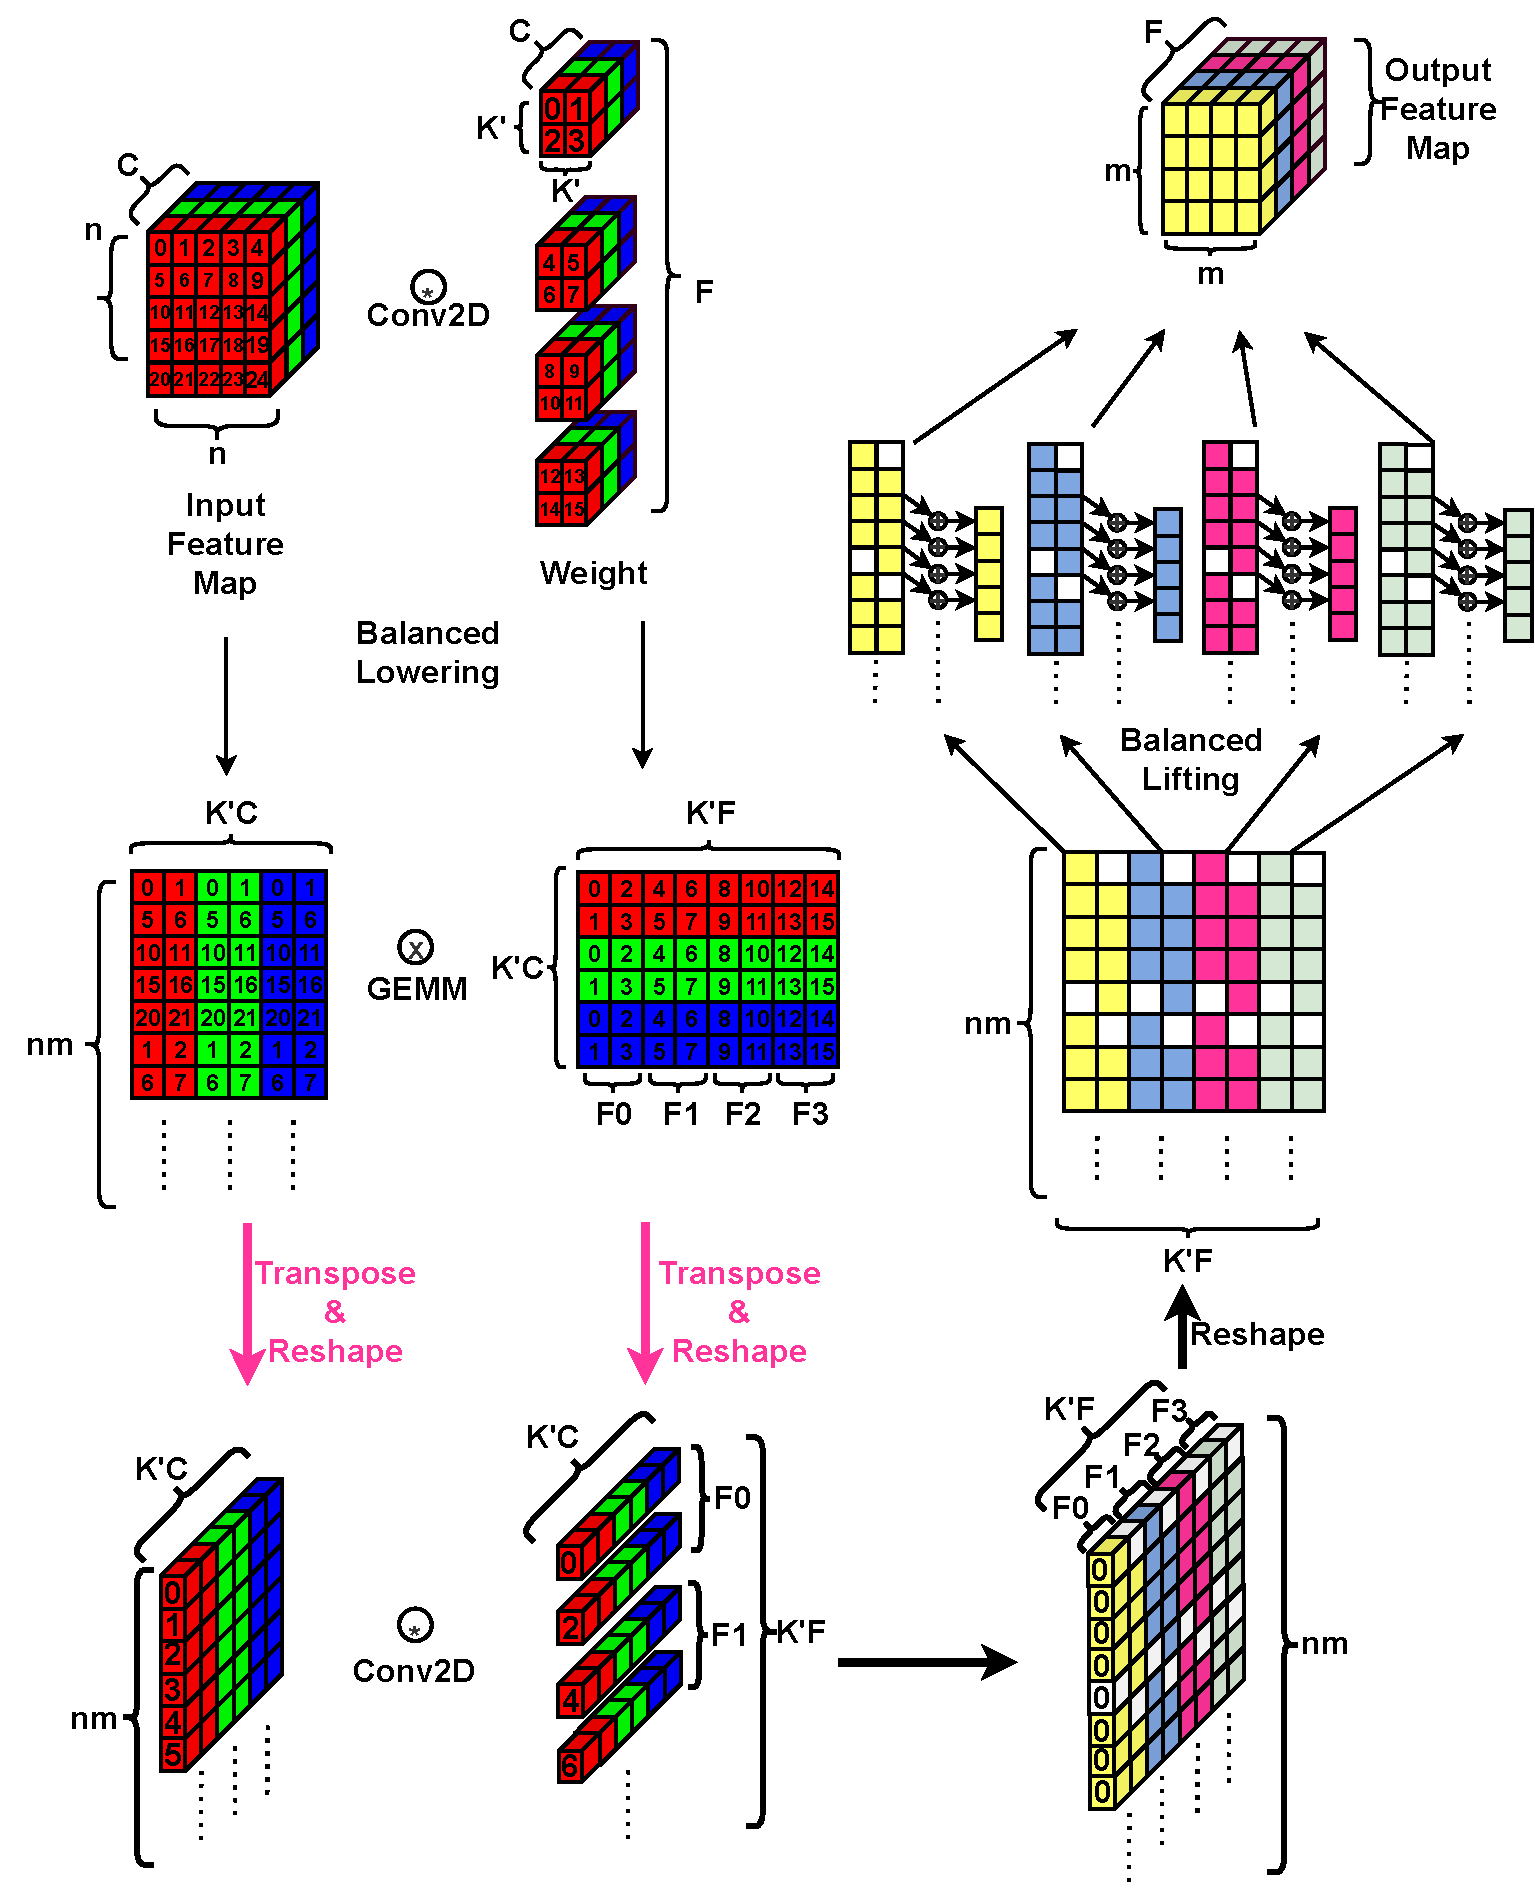
\includegraphics[scale=0.5]{fig/ConvToGemmToConv.pdf}
    \caption{Illustration of approach Conv2Gemm2Conv approach}
    \label{fig:conv2gemm2conv}
\end{figure}

\subsection{Layer Dimensionality}
\label{chap:dda:dataflow_dse:GEMM_mode:layer_dimentionality}

A convolution layer's kernel size being supported directly or
through GEMM mode has an effect on the assumed
dimensionalities of the IFmap and Weight tensors as well as the kernel loops
unroll factor K. Kernels are assumed to be symmetric so both kernel KY and KX
loops and share a single unroll factor $K_{unroll}$. If the convolution layer's
kernel size is supported directly no changes are assumed to have been made to
the dimensionality of the IFmap. The kernel unroll factor is then equal to the
kernel size of the layer in accordance with the conclusions drawn from
\autoref{chap:dda:dataflow_dse:pruning:applying_it}. However, if
a convolutions layer's kernel size is not supported directly, the layer's kernel
size is converted to (1, 1) as seen in \autoref{math:K_unroll_factor} and lowering
is assumed to have been performed on IFmap and Weight tensors in accordance with
the approach discussed in \autoref{chap:dda:dataflow_dse:GEMM_mode:layer_equivelence}. For a convolution
layer with IFmap dimensionality $R^{C\times n\times n}$, Weight dimensionality
$R^{F\times C\times K\times K}$ and OFmap dimensionality $R^{F\times m\times m}$
the layer's new filter count $\hat{F}$, channel count $\hat{C}$, and IFmap
channel size $\hat{Z}$ values are reflected in \autoref{math:layer_equivelence}. 

\begin{align}
    \begin{gathered}
        K_{unroll} = \begin{cases} K & K \in \{SupportedKernels\}\\1 &K \notin \{SupportedKernels\}\end{cases}
            \end{gathered}
    \label{math:K_unroll_factor}
\end{align}

\begin{align}
    \begin{gathered}
        \hat{C} = \begin{cases} C &  K \in \{SupportedKernels\}\\ CK & K \notin \{SupportedKernels\}\end{cases} \\
        \hat{F} = \begin{cases} F &  K \in \{SupportedKernels\}\\ FK & K \notin \{SupportedKernels\}\end{cases} \\
        \hat{Z} = \begin{cases} m^2 &  K \in \{SupportedKernels\}\\ nm & K \notin \{SupportedKernels\}\end{cases}
            \end{gathered}
    \label{math:layer_equivelence}
\end{align}

% \subsection{Overhead of lowering and lifting}
% \label{chap:dda:dataflow_dse:GEMM_mode:overhead}

Lowering and lifting introduce additional overheads with regards to latency and
tensor sizing. The latency for performing balanced lowering and lifting is
$m^{2}K$ for a layer with a Weight tensor $\mathbb{R}^{F\times C\times K\times
K}$ and an OFmap tensor $\mathbb{R}^{F\times m\times m\times}$. While lowering
and lifting can be performed by a convolutions accelerator, in this thesis it is
assumed that a software processor on the same chip performs these operations.
Lowering also introduces duplicate data elements in the IFmap tensor thus
increasing it's overall size. 

To enable GEMM operations using the approach in
\autoref{chap:dda:dataflow_dse:GEMM_mode:conv_gemm_equiv:proof} both input
and output matrices are transposed and reshaped. All reshape operations
discussed in this chapter add a dimension of size 1 to the data and they incur
no data reorganization overhead. Additionally, all transpose operations are
assumed to be performed during transfer to and from accelerator on-chip and thus
incur no latency penalty. A discussion of how transfers to and from on-chip
memory can mask the latency of transposing matrices is left as part of future
work along with incorporating lowering and lifting into the accelerator. 


\section{Exploring the Hardware Implementation Design Space}
\label{chap:dda:hw_dse}

Based on the conclusions derived from \autoref{chap:dda:dataflow_dse:pruning},
weight stationary is the most flexible dataflow choice given the overlap between
1x1 convolutions and GEMM discussed in
\autoref{chap:dda:dataflow_dse:GEMM_mode}. This gives rise to a weight
stationary dataflow based accelerator with two operational modes, direct Mode
where a subset of possible kernel sizes are supported directly and GEMM mode where all
other kernel sizes and strides are supported via the lowering/ lifting based
approach. 

In this section we will determine an appropriate on chip communication
infrastructure as well as the memory hierarchy for HERO using the hardware
implementation taxonomy from \cite{maestro} in tandem with a reuse analysis of
the different data elements in the weight stationary dataflow determined by the
previous section. To perform this reuse analysis we will use the polyhedral
model to analyze temporal reuse in \autoref{chap:dda:hw_dse:temporal_analysis}
and spatial reuse in \autoref{chap:dda:hw_dse:spatial_reuse_analysis} of data
elements in a convolution operation. Based on the analyzed reuse behavior an
initial hardware implementation for HERO will be given and further improved
after applying a simplification of the on-chip memory hierarchy in
\autoref{chap:dda:hw_dse:simplifying_hierarchy}. The final hardware
implementation for HERO will be given in \autoref{chap:dda:hw_dse:final}. Note
that the implementation in \autoref{chap:dda:hw_dse:final} will serve as
template to be further tuned based on a library of target networks in
\autoref{chap:arch_dimensioning}.  

\subsection{Temporal Reuse Analysis}
\label{chap:dda:hw_dse:temporal_analysis}

Unrolling convolution dataflow loops yield multiple instances of the \ac{MAC}
statement across different loops present in the original convolution nested loops in
\autoref{lst:conv_loop}. These statements represent \ac{PE}s performing MAC
operations concurrently. Since there are no data dependencies between the MAC
statements across different unrolled loop instances all of the MAC statements
can be fused into one larger loop body as seen in \autoref{lst:conv_loop}.
\ac{MAC} statement instances can be distinguished from each other based on the memory access offsets that
exist in them as a result of unrolling filter, channel and kernel loops. For
unroll factors F\_T for filters, C\_T for channels, KY\_T and KX\_T for kernels
each statement will have a corresponding access offset based on the statement
index $j \in [0, F\_T*C\_T*KY\_T*KX\_T]$ for each of the data elements
(IFmap, OFmap and Weights) accessed in the loop body. Each \ac{MAC} statement
at index j is characterized by a set of access offsets {Fj, Cj, KYj,
KXj} used by the memory accesses in the \ac{MAC} statement. Applying the unroll
factors and distinguishing each \ac{MAC} statement based on it's statement index
j yields the loop configuration in \autoref{lst:conv_loops_unrolled}. 

\clearpage 

\begin{lstlisting}[language=C, caption=Fully unrolled convolution dataflow loops, label={lst:conv_loops_unrolled}]
    for(int f = 0; f < F; f+=F_T) // Filter loop
        for(int c = 0; c < C; c+=C_T) // Channel loop
            for (int y = 0; y < Y; y++) // FeatureMap Height
                for(int x = 0; x < X; x++) // FeatureMap Width
                        ...
                        /* For all j in [0, F_T*C_T*KY_T*KX_T[ */ 
                        O[f+Fj][y][x] += W[f+Fj][c+Cj][KYj][KXj]* \
                                            I[c][y+KYj][x+KXj] 
                        ...
\end{lstlisting}

Each MAC statement is composed of three separate memory accesses for IFmap,
OFmaps and weights. For each of those memory access has a temporal index (it's location in time) defined by the
iteration domain vector $[f, c, y, x, ky, kx]$. A mapping exists between each
iteration domain vector and MAC statement's memory accesses.  
Temporal reuse analysis for each of the memory accesses in the MAC statements is performed on the loops in \autoref{lst:conv_loops_unrolled}. The different
operational modes (Direct/ GEMM) are analyzed concurrently using the same loop
representation as they only differ based on whether we set the width loop
upper bound to 1, and set the kernel loops upper bounds to 1. Since
kernel loops are always unrolled fully this sets KY\_T and KX\_T to 1. We can
analyze temporal reuse in the dataflow represented in
\autoref{lst:conv_loops_unrolled} by adapting the approach in \cite{meeus} 
to the aforementioned dataflow iteration domain and access functions.
Given iteration domain restrictions imposed by the polyhedral model,
\autoref{lst:poly:analysis} assumes unroll factors F\_T =
C\_T = 4. Setting F\_T and C\_T to concrete values does not change the reuse
behavior during temporal reuse analysis and conclusions regarding temporal reuse
that arise from setting F\_T = C\_T = 4 can still be generalized to other values.

\clearpage
\begin{lstlisting}[caption=Polyhedral analysis of reuse in iscc for convolution loops, label={lst:poly:analysis}]
    // Define iteration domain for all accessed data elements
    ID:=[F, C, Y, X] -> { S[f, c, y, x] : 0<=f<F and 0<=c<C and f mod 4=0 and c mod 4=0, 0<=y<Y and 0<=x<X};
    // Define access functions for each data element
    IFmap:=([Cj, KYj, KXj] -> {S[f, c, y, x] -> IF[c+Cj][y+KYj][x+KXj]})*ID;
    OFmap:=([Fj] -> {S[f, c, y, x] -> PS[f+Fj][y][x]})*ID;
    WEIGHT:=([Fj, Cj, KYj, KXj] -> {S[f, c, y, x] -> W[f+Fj][c+Cj][KYj][KXj]})*ID;
    // Evaluate temporal reuse
    IFmap_REUSE:=(IFmap.(IFmap^-1))*(ID<<ID);
    OFmap_REUSE:=(OFmap.(OFmap^-1))*(ID<<ID);
    WEIGHT_REUSE:=(WEIGHT.(WEIGHT^-1))*(ID<<ID);  

\end{lstlisting}

In \autoref{lst:poly:analysis}, the iteration domain for the loops in
\autoref{lst:conv_loops_unrolled} is converted into it's set representation in
line 2 where for some access statement S the loop iteration vector [f, c, y, x,]
is bound by the upper and lower bounds [0, F], [0, C], [0, Y], [0, X]
respectively. These bounds are represented by the associated parameters passed
to the iteration domain set assignment in line 2. 

Each memory accessed for IFmaps, OFmaps and weights in each MAC statement has
an associated memory access function. 

Each instance of the loop iteration vector [f, c, y, x]
is mapped to a memory access for each of the memories in lines 4-6. Access
offsets used in the memory access functions are passed as parameters based on
the convention established in \autoref{lst:conv_loops_unrolled}. This mapping
creates multiple temporal instances for each memory access in each \ac{MAC}
statement instance.  For
example, the OFmap access that occurs at iteration vector [f = 2, c= 1, y = 0,
x = 1] is a different temporal instance of the same OFmap access at [f = 1, c = 1,
y = 0, x = 1]. 
Two accesses that access the same index but at different
iteration vectors are different temporal instances of the same access.
After applying the operation in lines 8-10, we can determine the
temporal reuse behavior of the accessed memories in the convolution loops.  
\autoref{lst:poly:result} shows the reuse behavior for each memory. Original
iteration domains constraints are omitted for brevity. The operation in lines
8-10 map all iteration domains to all proceeding iteration domains that access
the same memory locations for each of the data elements.

\clearpage
\begin{lstlisting}[caption=Polyhedral analysis results w.r.t data elements in convolution loops, label={lst:poly:result}]
    IFmap_REUSE;
    [F, C, Y, X, Cj, KYj, KXj]->{
        S[f, c, y, x] -> S[f', c' = c, y' = y, x' = x] :
            ... f' > f and 0 <= f' < F ... 
        }
    OFmap_REUSE;
    [F, C, Y, X, Fj]->{ 
        S[f, c, y, x] -> S[f' = f, c', y' = y, x' = x] : 
            ... c' > c and 0 <= c' < C ... 
        }
    WEIGHT_REUSE;
    [F, C, Y, X, Fj, Cj, KYj, KXj] -> { 
        S[f, c, y, x] -> S[f' = f, c' = c, y', x'] : 
            ... y' > y and 0 <= y' < Y and 0 <= x' < X ...; 
    }
\end{lstlisting}

\autoref{lst:poly:result} shows the temporal reuse behavior in memory accesses. For each
of the memories accessed (IFmap, OFmap and Weights) there exists a set of reuse
(IFmap\_REUSE, OFmap\_REUSE and WEIGHT\_REUSE) maps that map each iteration
vector of an access to all the proceeding iteration vectors where that same
access occurs. From the above listing we can see that, in the set of IFmap reuse
maps (IFmap\_REUSE), IFmap channels are reused temporally with respect to filter
loops. For a given IFmap accessed at channel c, that channel is accessed again
when computing the output for all proceeding filter loop iteration f' where
$f'>f$. The absence of other mappings in the set of reuse maps IFmap\_REUSE shows
that 1) this reuse behavior holds at any arbitrary iteration vector [f, c, y, x]
and 2) this reuse behavior depends only on the filter loop. For the set OFmap
reuse maps (OFmap\_REUSE), for an OFmap access at iteration vector [f, c, y,
x], it is accessed again at loop iteration f'=f, c', y'=y, x'=x where $c'>c$.  
For (WEIGHT\_REUSE) Weights exhibit temporal reuse w.r.t feature map width and
height, the X and Y loops. 

Applying the hardware taxonomy in \cite{maestro}, IFmap exhibits temporal reuse,
multicast communication given their repeated read only behavior. OFmap exhibits temporal reuse, reduction communication
given their read-modify-write behavior. Weights exhibit temporal multicast
communication. Given the limited implementation options derivable from temporal
reuse we can comfortably define the appropriate connectivity and memory
hierarchies for IFmaps channels, OFmaps channels (equivalent to number of
Filters), and Weights. The beginnings of a hardware template derived from the
aforementioned temporal reuse behavior of the different memories referenced in
the convolution dataflow can be seen in \ref{fig:reuse_illus}. In
\ref{fig:reuse_illus} the template is broken into 3 major components. The first
is the IFmap memory hierarchy currently with only 1 level. The 2nd component is
the compute portion of the template where partial sums are computed and
aggregating into OFmap data elements. Finally the 3rd component which is the
OFmap memory that stores OFmap partial sums until they are aggregated into OFmap
pixels and are written back to memory.

\begin{figure}[]
    \centering
    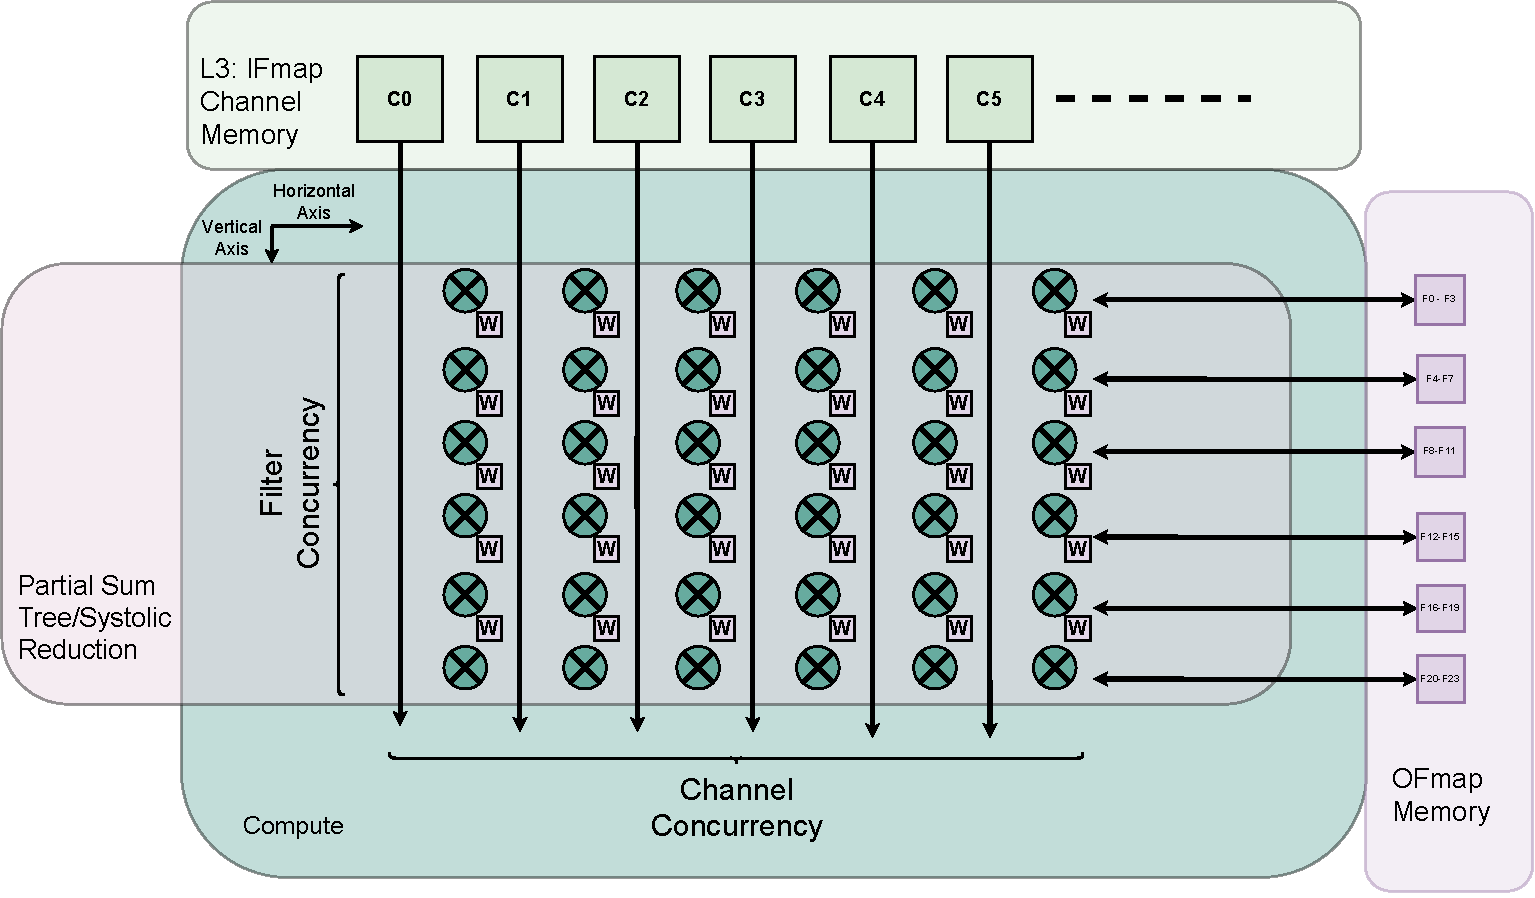
\includegraphics[scale=0.4]{fig/reuse_illus.pdf}
    \caption{Initial hardware template incorporating buffers IFmap and OFmap temporal reuse}
    \label{fig:reuse_illus}
\end{figure}

In addition to the temporal reuse behavior exhibited across IFmap channels,
temporal reuse exists within individual IFmap channels due to the stencil based
access pattern arising from the X, Y, KY, KX loops in the dataflow. That
temporal reuse is affected by the decision to fully unroll kernel loops which
causes temporal reuse to exist between unrolled different PEs processing the
same kernel. Proof of the existence of that temporal reuse is given in the polyhedral analysis in
\autoref{lst:poly:xy_reuse}. 

\begin{lstlisting}[caption=Analysis of IFmap channel reuse, label={lst:poly:xy_reuse}]
    ID_XY:=[Y, X, KY, KX] -> { S[y, x, ky, kx] : 0<=ky<KY and 0<=kx<KX and 0<=y<Y and 0<=x<X};
    IFmap_XY:=({S[y, x, ky, kx] -> IF[y+ky][x+kx]})*ID;
    IFmap_REUSE_XY:=(IFmap_XY.(IFmap_XY^-1))*(ID_XY<<ID_XY);
    IFmap_XY_REUSE;
    [Y, X, KY, KX] -> { 
        S[y, x, ky, kx] -> S[y', x', ky' = (y - y') + ky, kx' = (x - x') + kx] : 
            ... y' > y and (y + ky) -KY < y' <= (y + ky) and (x + kx) -KX < x' <= (x + kx) ...;}
\end{lstlisting}

\begin{figure}[]
    \centering
    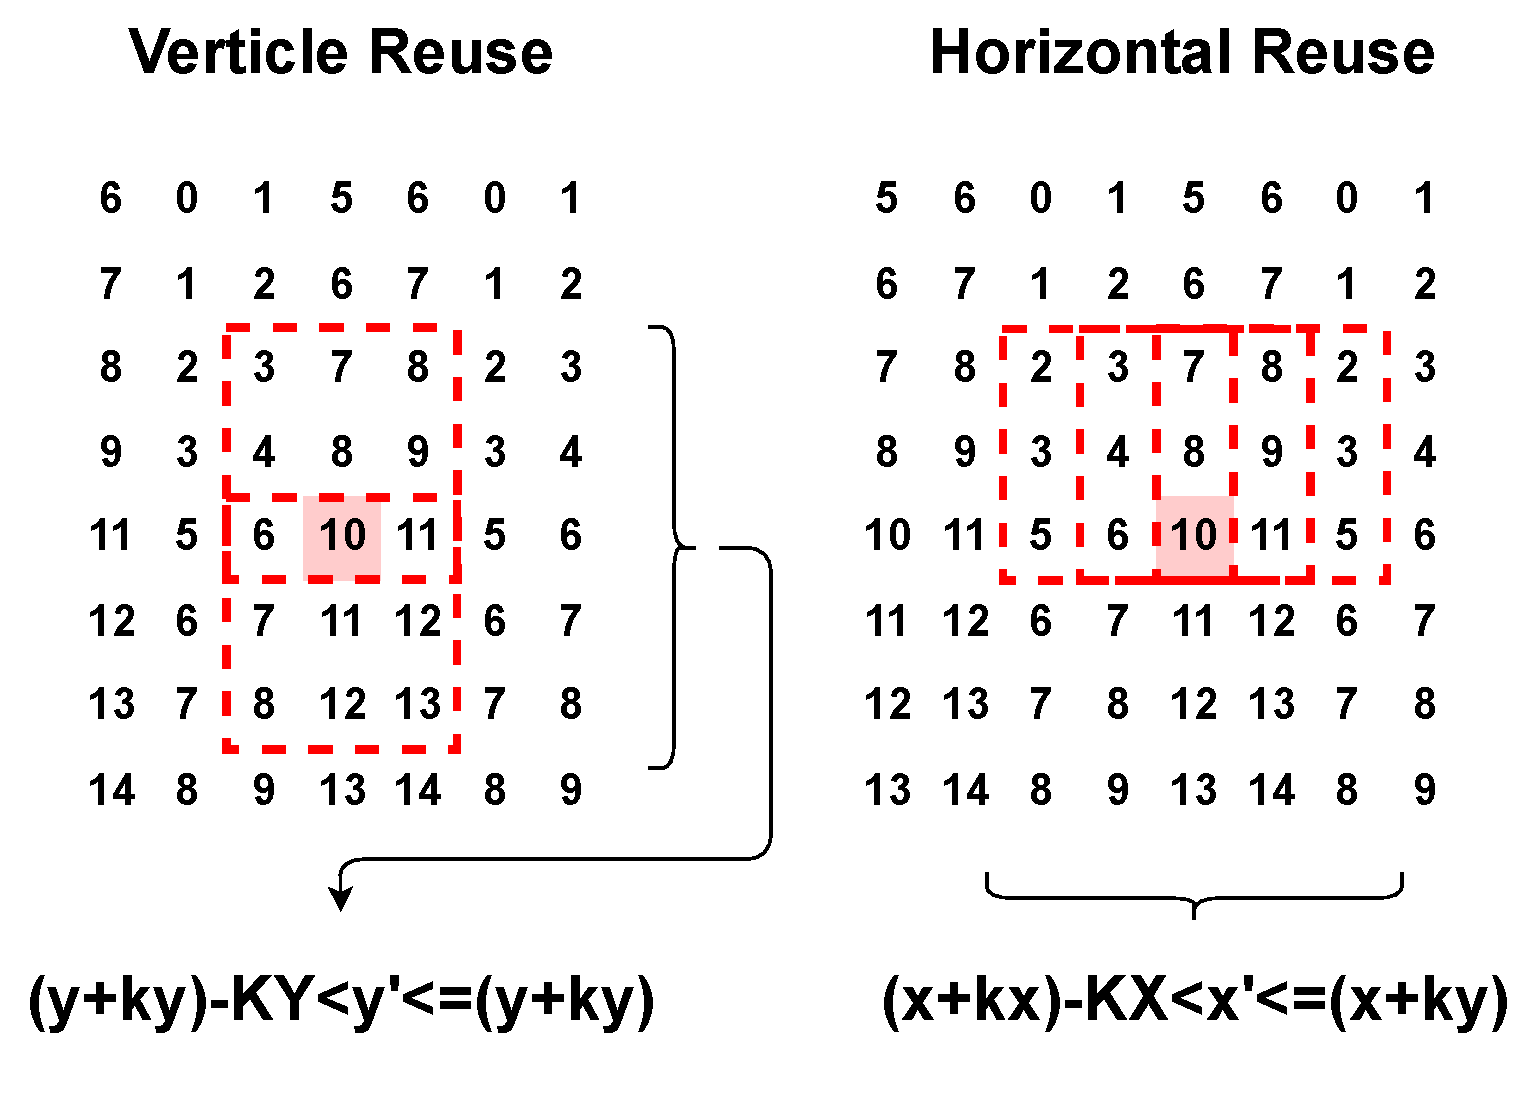
\includegraphics[scale=0.8]{fig/xy_reuse.pdf}
    \caption{IFmap Reuse Behavior w.r.t individual feature map channels}
    \label{fig:IFmap_xy_reuse}
\end{figure}

Within an individual IFmap channel, temporal reuse is exhibited w.r.t X and Y
loops. Given the complexity of the domain constraints of IFmap\_XY\_REUSE in
\autoref{lst:poly:xy_reuse}, an illustration of the reuse behavior is available
in \figref{fig:IFmap_xy_reuse}. In \figref{fig:IFmap_xy_reuse}, individual
pixels within the kernel are reused based on the position of the sliding window
or stencil of the convolution in an IFmap channel. There are two primary
directions where that reuse is exhibited, vertical and horizontal with an IFmap
channel. The loops that control the vertical and horizontal stencil position in
the IFmap are the Y and X loops in the dataflow. Because kernel loops are fully
unrolled, the temporal reuse exhibited in \autoref{lst:poly:xy_reuse} occurs
across different PEs processing the unrolled kernel. To determine the appropriate memory
infrastructure to support that stencil based access pattern, we can apply the
technique in \cite{meeus} to construct a reuse chain that moves reused data
between different PEs. The advantage of using a reuse chain is that the
temporal reuse that exists within an IFmap channel is relegated to a smaller
memory with lower memory access cost.

\cite{meeus} constructs a reuse chain for applications with a sliding window
access pattern that connects each unrolled kernel port with it's neighbors using
a FIFO or a shift register. If the temporal reuse distances between the accesses
of neighboring PE ports are constant \cite{meeus} uses a shift register,
otherwise they use a FIFO. The reuse distance between accesses of neighboring
ports are then converted into storage of the same size. So if two ports share
the same data but with a lag of 2 iterations in the iteration domain they're
operating in, then a shift register of size 2 can be placed between them.
Similar to the sliding window application explored in \cite{meeus} the reuse
distances between the PEs processing the unrolled kernel in the convolution
dataflow are also constant. To determine the reuse distances necessary between
ports we can apply the analysis in \autoref{lst:poly:xy_buffer_sizing:analysis}
adapted from \cite{meeus} to determine the sizing of the buffers in the reuse
chain for IFmap accesses within a channel. The analysis in
\autoref{lst:poly:xy_buffer_sizing:analysis} assumes a kernel size of (3, 3) based
on the conclusions of
\autoref{chap:dda:dataflow_dse:pruning:applying_it:loop_unroll_factors}. Note
that (1, 1) kernels exhibit no temporal reuse within the kernel loops.  

\begin{lstlisting}[caption=Determining buffer sizes in 3x3 convolutions, label={lst:poly:xy_buffer_sizing:analysis}]
    ID:=[IFmap_Y, IFmap_X] -> {S[y,x]:y>=0 and x>=0 and y<=IFmap_Y-3 and x<=IFmap_X-3};
    A0:=[IFmap_Y, IFmap_X] -> {S[y,x]->A[y+0,x+0]}*ID;
    A1:=[IFmap_Y, IFmap_X] -> {S[y,x]->A[y+0,x+1]}*ID;
    A2:=[IFmap_Y, IFmap_X] -> {S[y,x]->A[y+0,x+2]}*ID;
    A3:=[IFmap_Y, IFmap_X] -> {S[y,x]->A[y+1,x+0]}*ID;
    ...
    A8:=[IFmap_Y, IFmap_X] -> {S[y,x]->A[y+2,x+2]}*ID;

    R10:=(lexmin ((A1.A0^-1)*(ID<<ID)));
    R21:=(lexmin ((A2.A1^-1)*(ID<<ID)));
    R32:=(lexmin ((A3.A2^-1)*(ID<<ID)));
    ...
    R87:=(lexmin ((A8.A7^-1)*(ID<<ID)));
\end{lstlisting}

In \autoref{lst:poly:xy_buffer_sizing:analysis}, the iteration domain for the YX
loops are defined as functions of the IFmap dimensions passed as parameters (line 1).
The unrolled kernel loop IFmap accesses are then described using access maps
that map the iteration vector [y,x] to the associated IFmap access (lines 2-7).
Notice that the accesses are described as constant offsets added to access iterators y
and x. These constants represent the kernel loop iterators ky, and kx that are now
unrolled. For each neighboring pair of ports accessing the IFmap we can
determine the reuse behavior in (lines 9-10). Operations in lines (9-13) map
iterations where a port accesses a data element in IFmap with the earliest next
iteration in which the neighboring port accesses that same data element. The
distance between the accesses is then used as the reuse buffer size. The results
of the analysis are presented in \autoref{lst:poly:xy_buffer_sizing:results}.

\clearpage 

\begin{lstlisting}[caption=Polyhedral analysis of reuse in iscc for convolution loops, label={lst:poly:xy_buffer_sizing:results}]
R10;
$1 := [IFmap_Y, IFmap_X] -> { 
    S[y, x] -> S[y' = y, x' = 1 + x] : 
        0 <= y <= -3 + IFmap_Y and 0 <= x <= -4 + IFmap_X 
}
R21;
$2 := [IFmap_Y, IFmap_X] -> { 
    S[y, x] -> S[y' = y, x' = 1 + x] : 
        0 <= y <= -3 + IFmap_Y and 0 <= x <= -4 + IFmap_X 
}
R32;
$3 := [IFmap_Y, IFmap_X] -> { 
    S[y, x] -> S[y' = 1 + y, x' = -2 + x] : 
        0 <= y <= -4 + IFmap_Y and 2 <= x <= -3 + IFmap_X 
}
...
R87;
$8 := [IFmap_Y, IFmap_X] -> { 
    S[y, x] -> S[y' = y, x' = 1 + x] : 
        0 <= y <= -3 + IFmap_Y and 0 <= x <= -4 + IFmap_X 
}
\end{lstlisting}

In \ref{lst:poly:xy_buffer_sizing:results}, reuse distances between neighboring
ports depend on the relationship between the ports and whether their access offsets
are in the same row of the stencil or not. If two neighboring ports have unequal
ky offsets the reuse distance between them is IFmap\_X-3. If two neighboring
ports have an equal ky offset the reuse distance is 1. An example of the first
case is lines 11-15 where the reuse distance between port 2 and port 3 is
IFmap-3. The evidence of that is that for any data accessed at port 3 with
iteration vector y, x that same data is accessed at port 2 at iteration vector
[y+1, x-2]. Based on the lexicographic ordering of iteration vector [y, x] and [y+1,
x-2], the distance between those two vectors is IFmap\_X-3, or in terms of OFmap
dimensions X-1. Applying the same analysis to two ports in the same row (R10,
R21, R45, R87, ...) yields a reuse distance of 1 as evidence by the iteration
vectors of access [y, x] and [y, x+1] in all of the aforementioned neighboring
port pairs. 

Applying the results of the analysis in
\autoref{lst:poly:xy_buffer_sizing:results} with the previous template \autoref{fig:reuse_illus}
results in the updated template \autoref{fig:reuse_chain}.

\begin{figure}[]
    \centering
    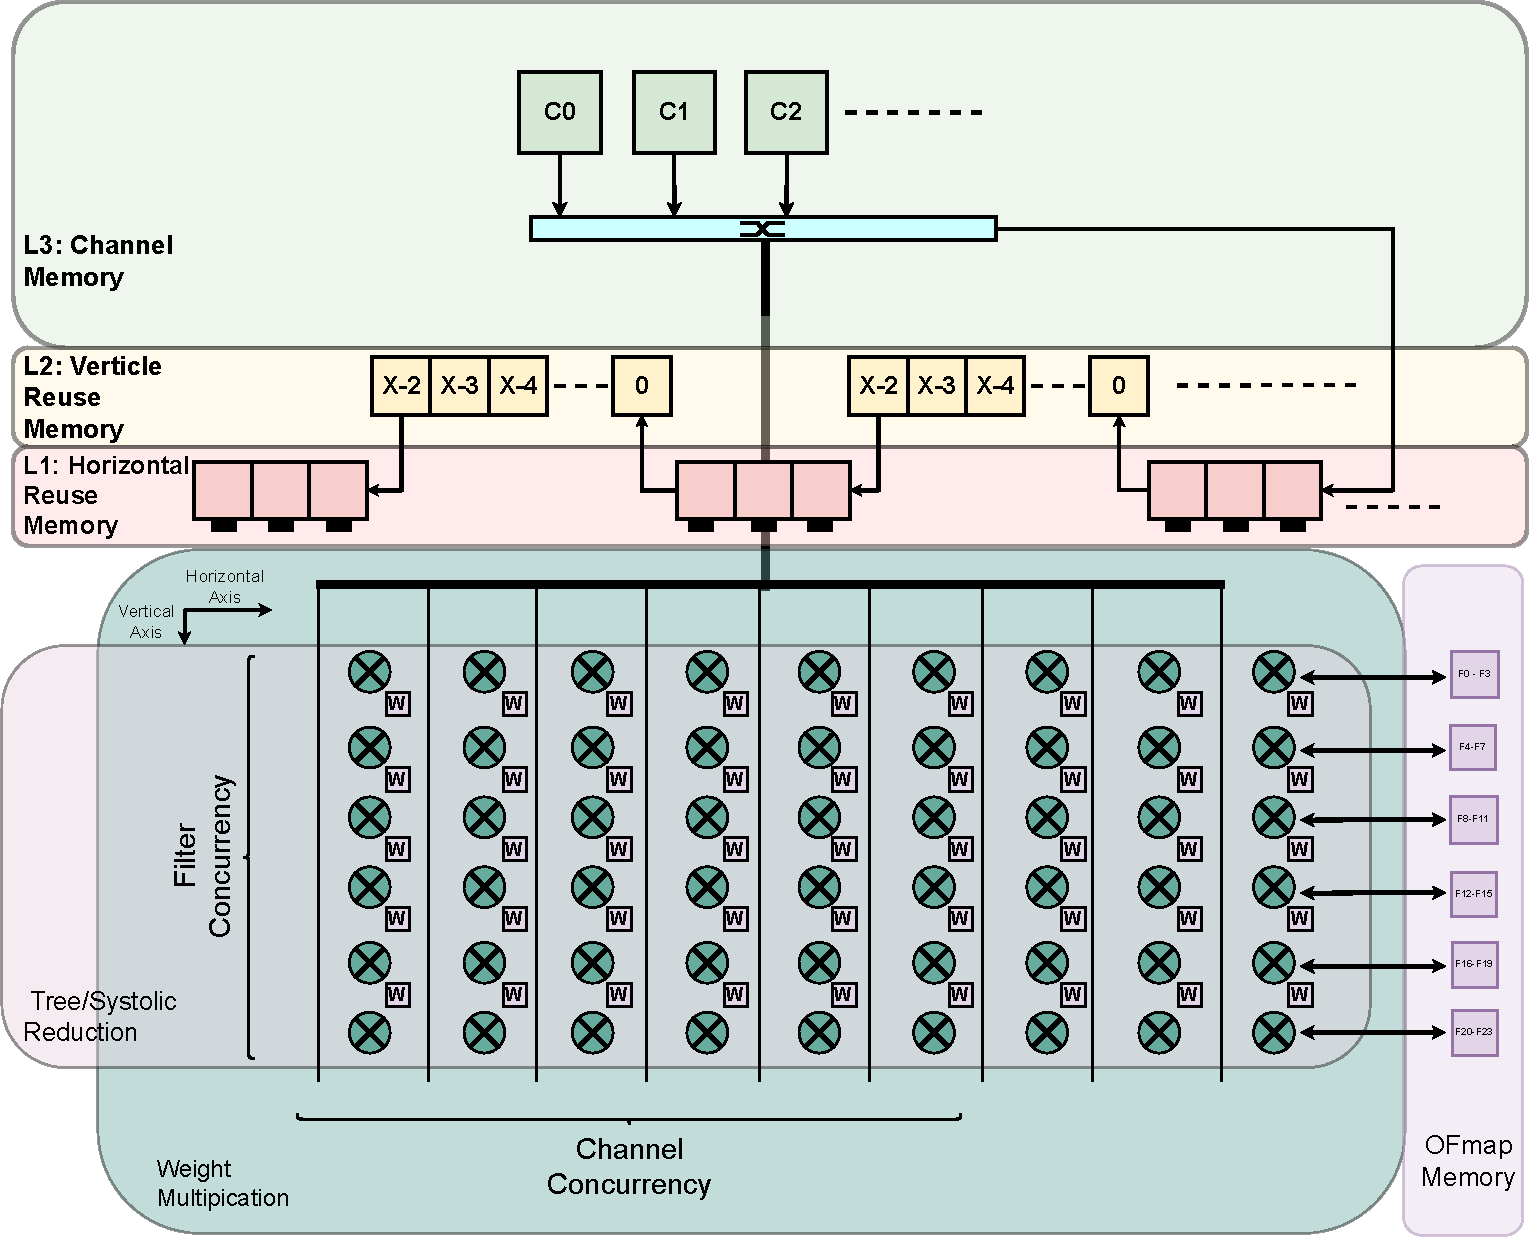
\includegraphics[scale=0.4]{fig/reuse_chain.pdf}
    \caption{Hardware template incorporating a reuse chain for reuse within an IFmap channel }
    \label{fig:reuse_chain}
\end{figure}


\subsection{Spatial Reuse Analysis}
\label{chap:dda:hw_dse:spatial_reuse_analysis}

Each MAC statement in the unrolled loop body has an associated j index. In the
loop body there exists duplicate memory accesses across individual \ac{MAC}
statements. Those duplicate accesses are highlighted in
\autoref{lst:conv_loops_unrolled_fully} and they are the origin of spatial reuse
in the dataflow. IFmaps exhibit spatial reuse with multicast communication w.r.t
to filter loops. OFmap exhibit spatial reuse with reduction communication
w.r.t to channel loops. Weights exhibit no spatial reuse 
 
\clearpage
\begin{lstlisting}[language=C, caption=Spatial reuse in fully unrolled kernel loops, label={lst:conv_loops_unrolled_fully}]
for(int f = 0; f < F; f+=F_T) // Filter loop
    for(int c = 0; c < C; c+=C_T) // Channel loop
        for (int y = 0; y < Y; y++) // FeatureMap Height
            for(int x = 0; x < X; x++) // FeatureMap Width
            {
                %\colorbox{green}{O[f+0][y][x]}% += W[f+0][c+0][0][0] * \ 
                                    %\colorbox{yellow}{I[c+0][y+0][x+0]}%; // j=0
                %\colorbox{green}{O[f+0][y][x]}% += W[f+0][c+0][0][1] * \
                                    %\colorbox{yellow}{I[c+0][y+0][x+1]}%; // j=1
                %\colorbox{green}{O[f+0][y][x]}% += W[f+0][c+0][0][2] * \
                                    I[c+0][y+0][x+2];  // j=2
                %\colorbox{green}{O[f+0][y][x]}% += W[f+0][c+0][1][0] * \ 
                                    I[c+0][y+1][x+2];  // j=3
                ...
                %\colorbox{red}{O[f+1][y][x]}% += W[f+1][c+0][0][0] * \
                                    %\colorbox{yellow}{I[c+0][y+0][x+0]}%; // j=C_T*KY_T*KX_T
                %\colorbox{red}{O[f+1][y][x]}% += W[f+1][c+1][0][1] * \
                                    %\colorbox{yellow}{I[c+0][y+0][x+1]}%; // j=C_T*KY_T*KX_T+1
                ...
                O[f+F_T-1][y][x] += W[f+F_T-1][c+C_T-1][KY_T-1][KX_T-1] * \ 
                                        I[c][y+KY_T-1][x+KX_T-1]; 
                                                    // j=F_T*C_T*KY_T*KX_T-1
                                        
            }
\end{lstlisting}

Applying the taxonomy in \autoref{fig:hw_taxonomy} to data elements that are
spatially reused, IFmap channels that are spatially reused across unrolled
filter loops can be broadcast with a bus. The reuse chain discussed in
\autoref{chap:dda:hw_dse:temporal_analysis} can be thought of as a
Store\&Forward scheme to deliver individual IFmap channel data elements to the
\ac{PE}s for reduction into OFmaps.Weights reused for channel iteration and are
discarded. They exhibit no spatial reuse, just temporal. Therefore they should
be kept in small on chip buffers, preferably close to the computation they are
used in. OFmap exhibit spatial reuse across concurrent channels as well as
temporal reuse across channel sets as discussed in
\autoref{chap:dda:hw_dse:temporal_analysis}. A reduction tree as in
\autoref{fig:reduction_styles}.a or a systolic array reduce and fwd as in
\autoref{fig:reduction_styles}.b are both possible assuming no restrictions
arising from synthesis. Combining the reuse chain derived in
\autoref{chap:dda:hw_dse:temporal_analysis} with the required systolic
delays yields a simplification to the L1 memory present in
\autoref{fig:reuse_chain}. This simplification is discussed in
\autoref{chap:dda:hw_dse:simplifying_hierarchy}.


\begin{figure}
    \centering
    \subfigure[]{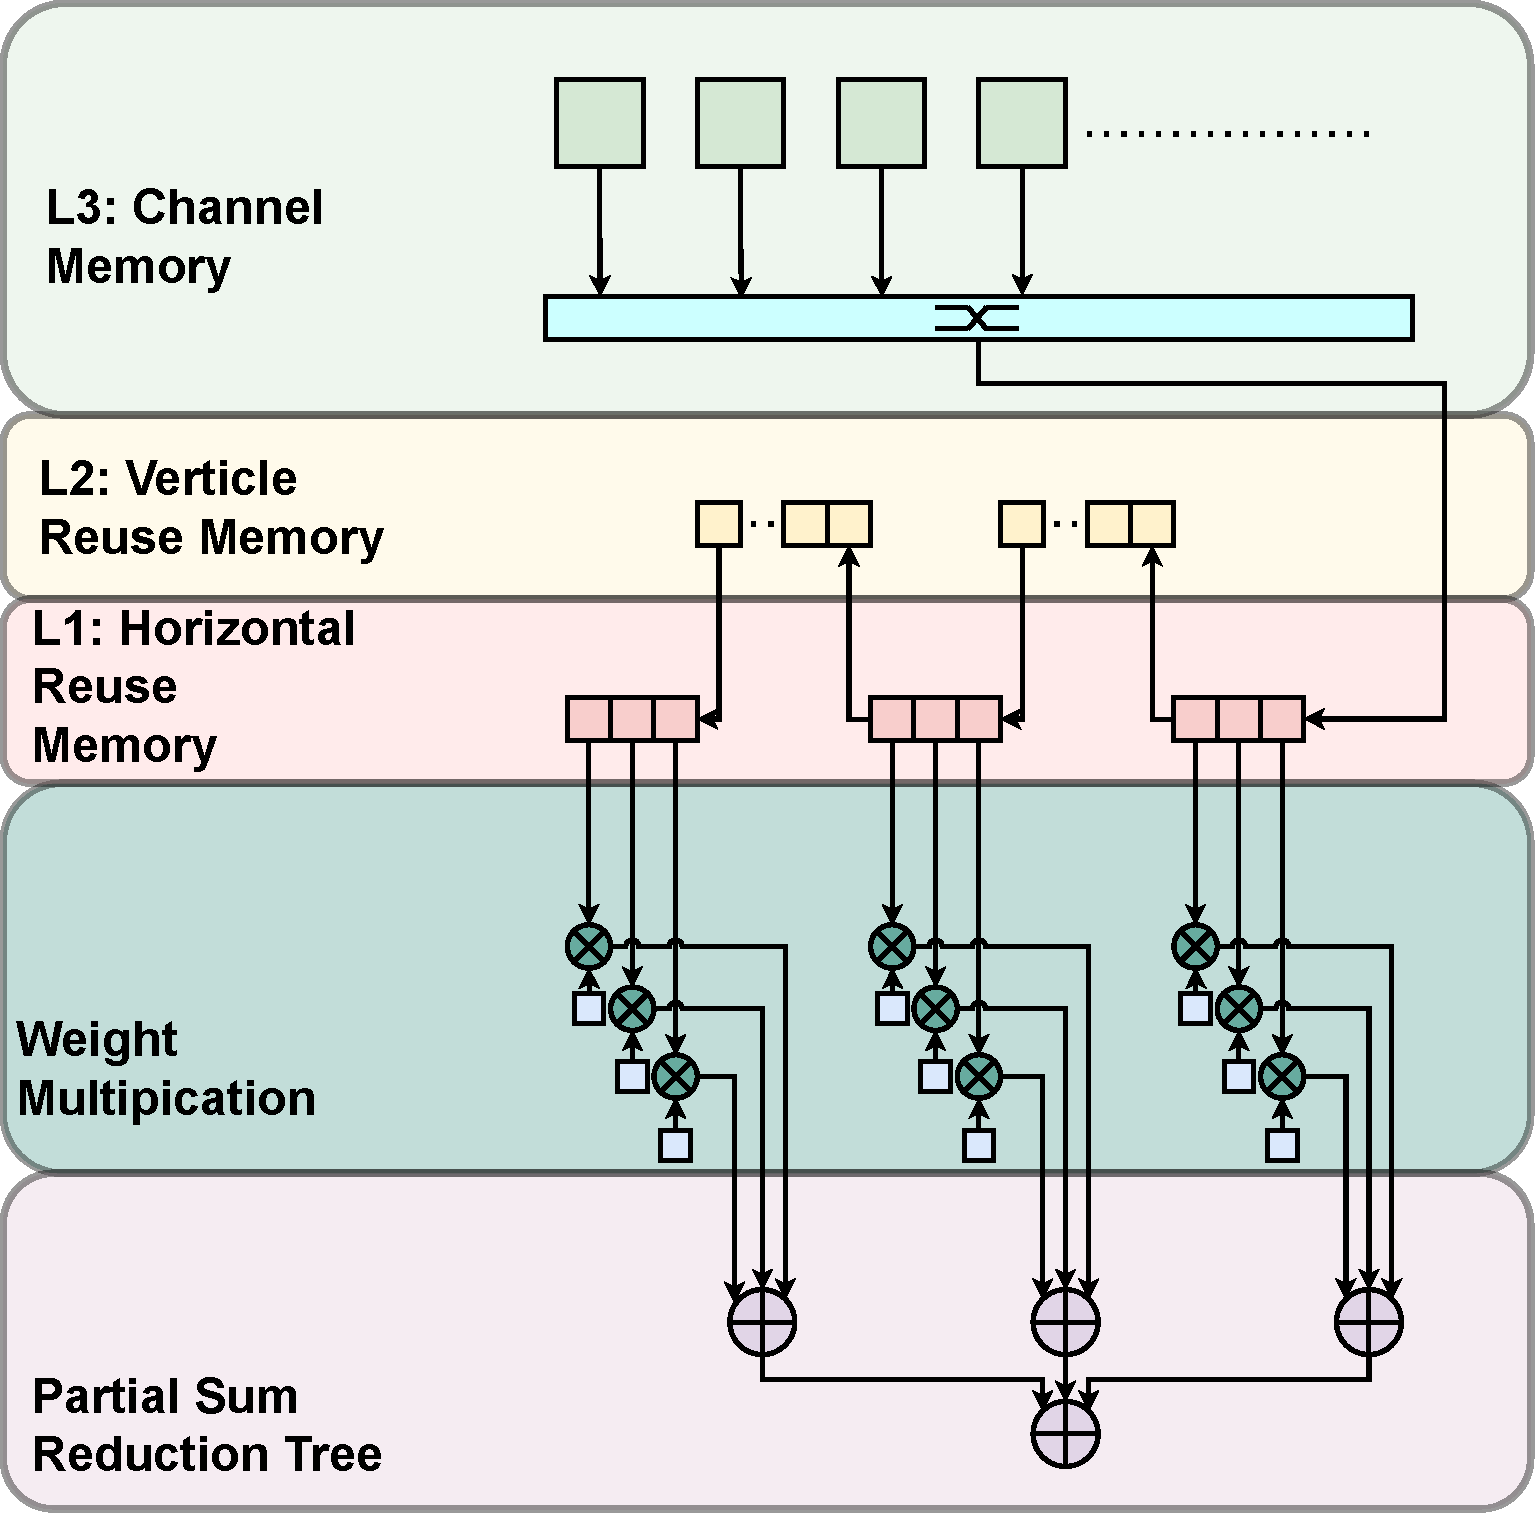
\includegraphics[width=0.5\textwidth]{fig/treeReduction.pdf}}
    \subfigure[]{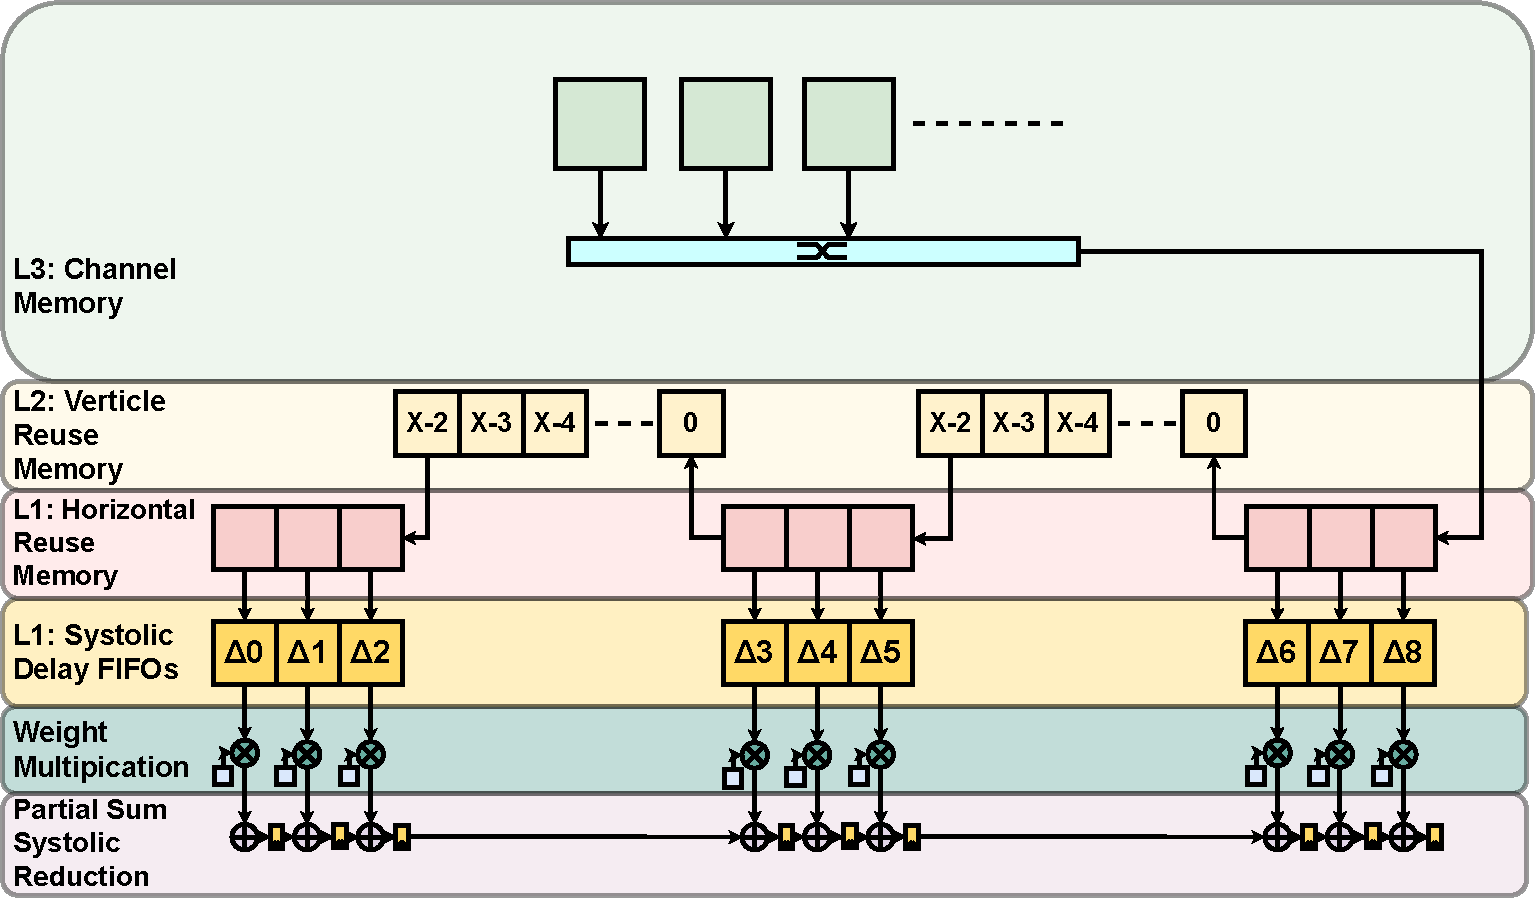
\includegraphics[width=0.7\textwidth]{fig/SystolicReduction.pdf}}
    \caption{Illustration of different partial sum reduction styles assuming kernel size is (3, 3) (a) Tree Reduction (b) Systolic array reduction}
    \label{fig:reduction_styles}
\end{figure}

\subsection{Simplifying the memory hierarchy}
\label{chap:dda:hw_dse:simplifying_hierarchy}

\begin{figure}[]
    \centering
    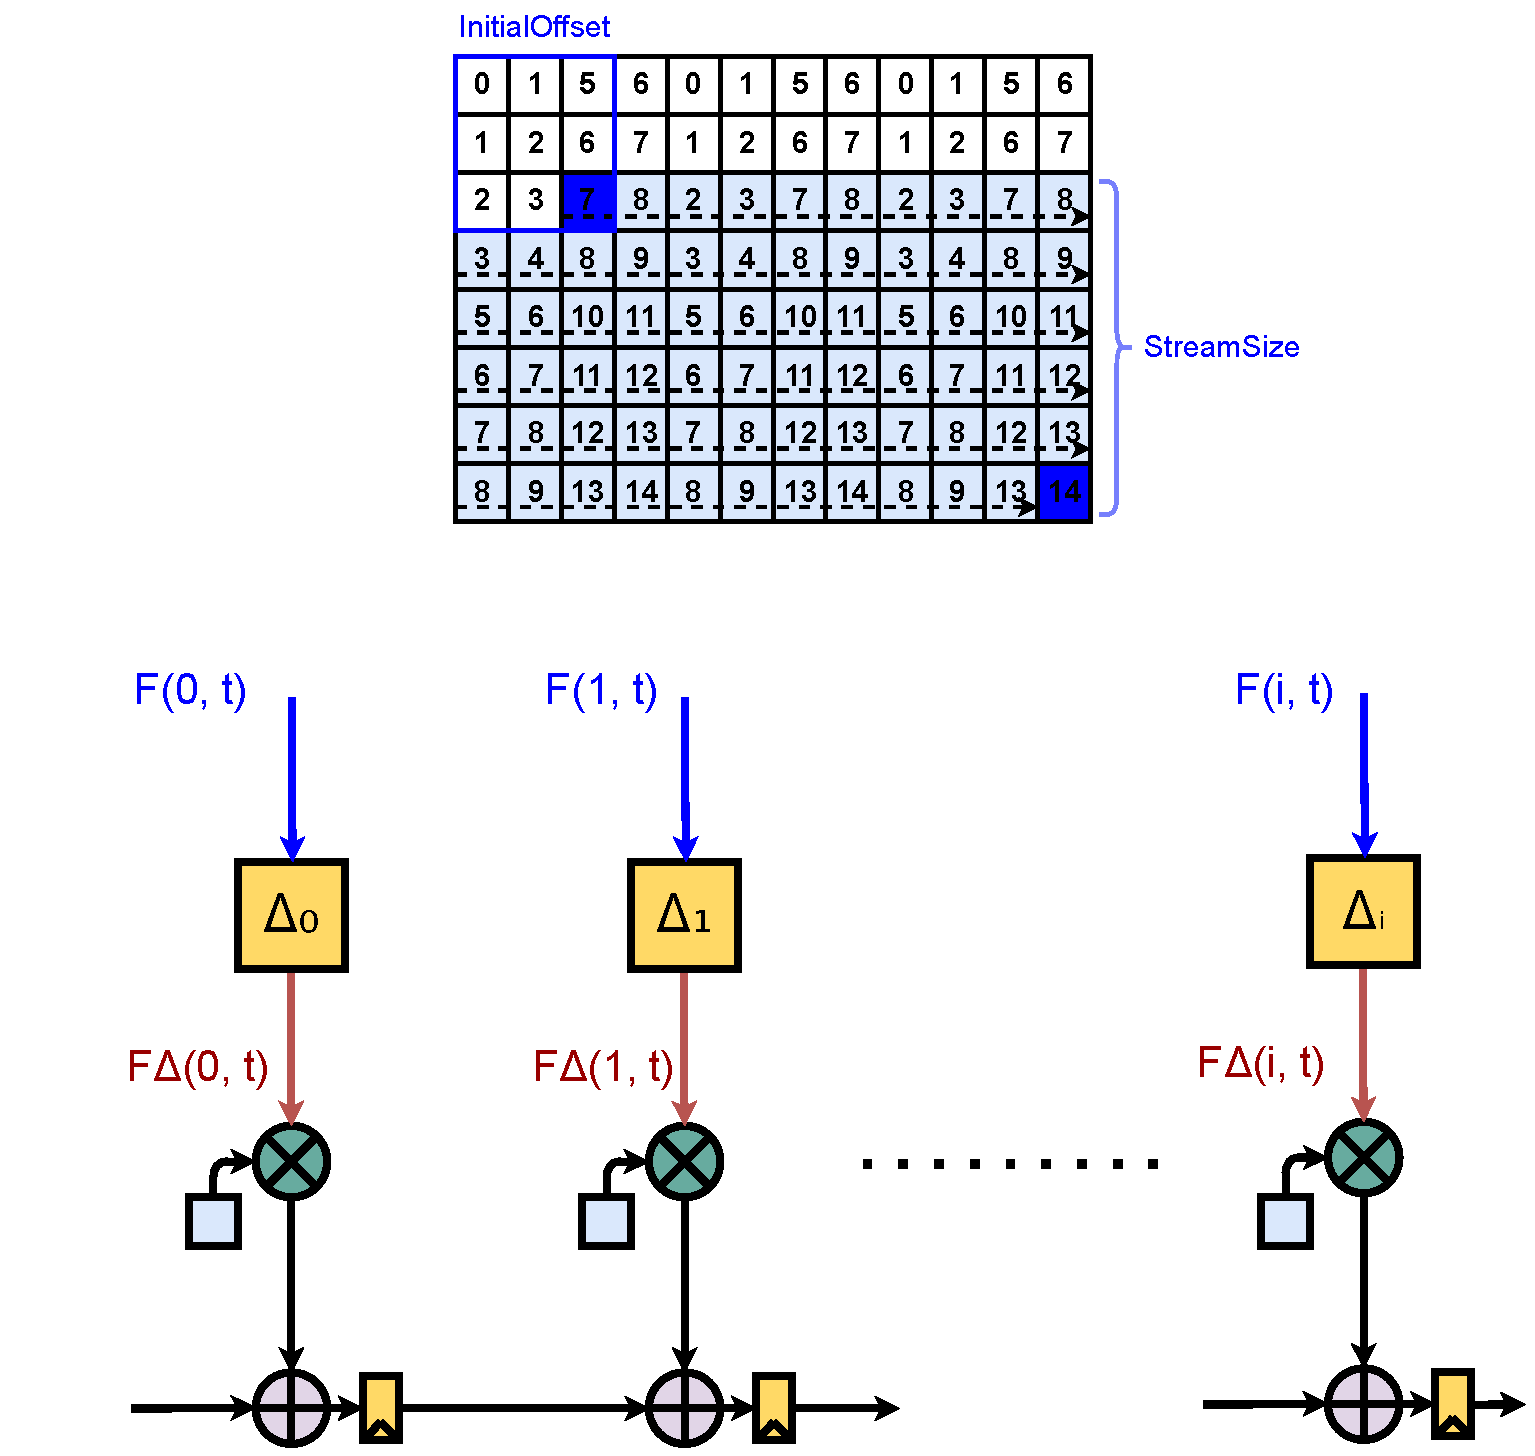
\includegraphics[scale=0.5]{fig/delayproof.pdf}
    \caption{Reinterpretation of IFmap memory hierarchy outputs as a stream function}
    \label{fig:delay_proof}
\end{figure}

We can reinterpret the accesses made by the IFmap memory hierarchy in
\autoref{fig:reuse_chain} as a stream function $F(i, t)$ whose output produces
element from an IFmap channel. The variable $i$ is the port index of the IFmap
hierarchy and $t$ is the time in cycles since the beginning of the convolution
operation. A representation of this reinterpretation of the accesses made in the
IFmap memory hierarchy can be seen in \autoref{fig:delay_proof}. Since it's
always assumed that in direct mode kernel loops are unrolled fully the number of
ports into the IFmap memory hierarchy is always a multiple of $K^2$ where $K$ is
the size of the kernel being processed in direct mode. 

\begin{gather}
    IFmap \in R^{C\times n \times n} \xrightarrow{Reshape} IFmap \in R^{1\times Cn^2} \\
    Weight \in R^{F\times C\times K \times K} \\
    F(i, t)=    \begin{cases}
                    IFmap[A(i, t)] & 0<=t < StreamSize \\
                    0 & else
                \end{cases} \\
    StreamSize = n(n-K)+(n-K) \\
    A(i, t) = InitialOffset(i) + t
\end{gather}

Each data element streamed from the IFmap depends on an access function that
also takes the same variables $i$ and $t$. Depending on the port index $i$ the
access function for each port is composed of an initial offset in the IFmap and
the current cycle count $t$. A total of $StreamSize$ elements are streamed the IFmap
memory hierarchy. The stream size is a function of the IFmap dimensions
and the kernel Size. 

\begin{gather}
    InitialOffset = C_in^2+Y_in+X_i \\
    C_i = \lfloor \frac{\lfloor \frac{i}{K} \rfloor}{K} \rfloor \\
    Y_i = (\lfloor \frac{i}{K} \rfloor ) \bmod K\\
    X_i = i \bmod K = (i - \lfloor \frac{i}{K} \rfloor K)
\end{gather}

The initial offset function defines the initial index
offset in the IFmap tensor where stream begins from for each port $i$. It can be
decomposed into three main offsets. A channel offset $C_i$, a row offset $Y_i$
and a column offset $X_i$. 

\begin{gather}
    F_\Delta(i, t) = \begin{cases}
    IFmap[A_\Delta(i, t)] & \Delta_i<=t < \Delta_i+ StreamSize \\
    0 & else
    \end{cases} \\
    \Delta_i = i \\
    A_\Delta(i,t) = A(i, t) - \Delta_i
    % \hat{OFmap}(j) = \displaystyle\sum\limits_{i=0}^{ub(i)} A_\Delta(i, j+i)
\end{gather}

Under this new streaming based interpretation of the accesses in the IFmap
memory hierarchy, the delay elements in the systolic reduction scheme in
\autoref{fig:reduction_styles}.b are represented as time shifts in the stream
function $F(i,t)$. These time shifts are represented in the new delayed access
function $A_\Delta(i, t)$.

\begin{gather}
    A_\Delta(i,t) =  C_in^2+Y_in+X_i + t- i\\
    A_\Delta(i,t) =  C_in^2+Y_in + \underbrace{(i - \lfloor \frac{i}{K} \rfloor K)}_{X_i} + t - i\\
    A_\Delta(i,t) =  C_in^2+Y_in + \underbrace{(- \lfloor \frac{i}{K} \rfloor K)}_{X'_i} + t
\end{gather}

\begin{figure}[]
    \centering
    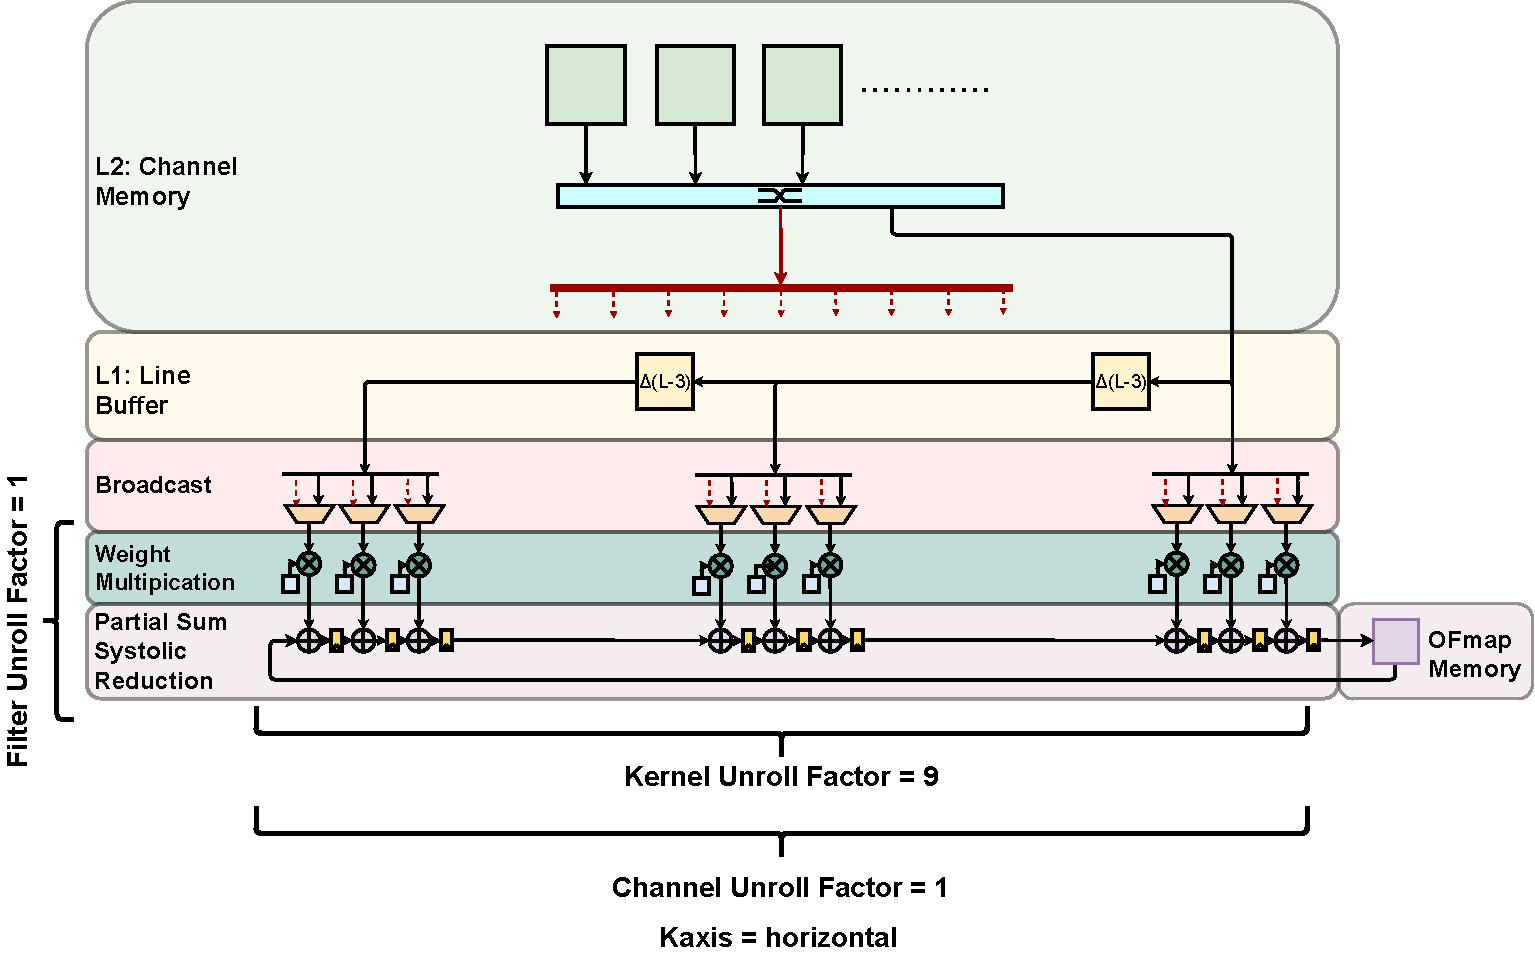
\includegraphics[scale=0.36]{fig/hybrid3x3Gemm.pdf}
    \caption{Using a systolic reduce and forward to calculate OFmaps}
    \label{fig:simplified_systolic_reduction}
\end{figure}

Substituting the InitialOffset function in $A_\Delta$  allows us to simplify the
column offset. This yields a new column offset $X'_i$. The final delayed access
function's initial offset becomes insensitive to changes in the port index $i$
that are not multiples of $K$. This allows us to remove the lowest layer memory
along with the systolic array delays in \autoref{fig:reuse_chain} and replace
both layers with just a series of broadcast buses that span consecutive $K$
groups of IFmap ports provided that we set the start time constraints to
$\Delta_i = \lfloor \frac{i}{K} \rfloor K$. Note that changing the start time
constraints will result in computing partial kernels that have invalid positions
within IFmaps and they must be discarded from the final output of the
accelerator. This simplification of the IFmap memory hierarchy by removing the
systolic delays still requires complex delayed reads from the IFmap hierarchy
which necessitates smart SRAMS whose access times can be programmed. A
discussion of these smart memories is presented in
\autoref{chap:data_orchestration}. The final hardware implementation with the
added IFmap memory hierarchy optimization discussed in this section is given in
\autoref{fig:simplified_systolic_reduction}.
\autoref{fig:simplified_systolic_reduction} shows the broadcast busses for every
group of 3 processing engines as well as the (1, 1) vertical broadcast busses
highlighted in red. 

\section{HERO: A Hybrid GEMM and Direct Conv. Accelerator}
\label{chap:dda:hw_dse:final}

After applying the simplification in
\autoref{chap:dda:hw_dse:simplifying_hierarchy} we arrive at the final HERO
template architecture variants in \autoref{fig:hero:horizontal} and
\autoref{fig:hero:vertical}. Both figures illustrate templates with unroll
factors for F, C loops undefined. Both variants in each of the figures represent
two different spatial axis mappings for the unrolled kernel loops. Depending on
the choice of axis mapping the effective channel concurrency available (in the
horizontal case in \autoref{fig:hero:horizontal}) and the effective number
filter concurrency available (in the vertical case in
\autoref{fig:hero:vertical}) for (1, 1) convolutions will change. A flexible
any-to-any interconnect that allows arbitrary bank access is assumed to exist for
both L3 IFmap memory and OFmap memory. Arbitrary access to any IFmap and OFmap
bank enables flexible distribution of IFmap and OFmap data across multiple
banks. The benefit of this flexible distribution will be discussed in
\autoref{chap:net_compile}. In addition to arbitrary IFmap bank access in
\autoref{fig:hero:horizontal}, the IFmap interconnect enables broadcasting of
IFmap pixels vertically to all filters rows in HERO as well as broadcasting
IFmap pixels across groups of PEs for (3, 3) kernel computations. The choice of
which spatial axis mapping and F and C unroll factors is discussed further in
\autoref{chap:arch_dimensioning} where these HERO template parameters are
optimized based on the layer configurations present in the TIMM Library's
networks.   

\begin{figure}[ht]
    \centering
    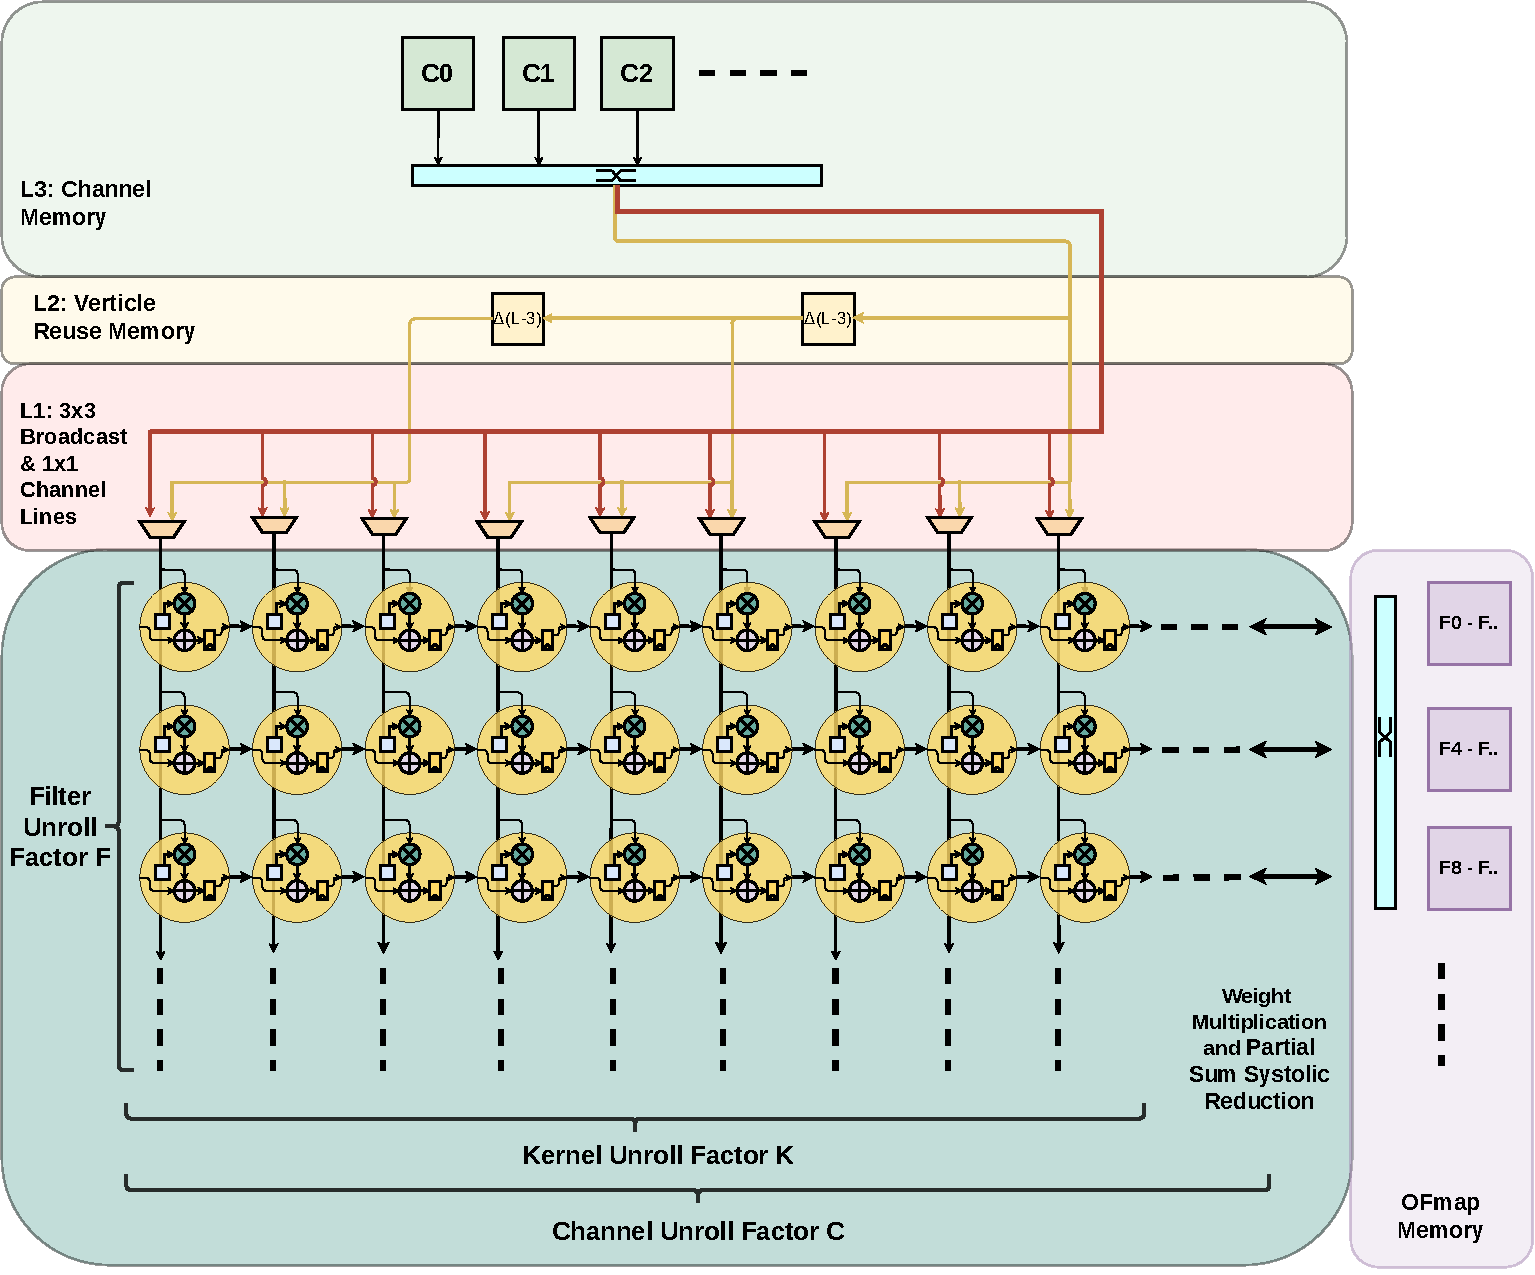
\includegraphics[scale=0.58]{fig/hero-t-horizontal.pdf}
    \caption{HERO template with both Kernel and Channel loops mapped to the horizontal axis}
    \label{fig:hero:horizontal}
\end{figure}

\begin{figure}[ht]
    \centering
    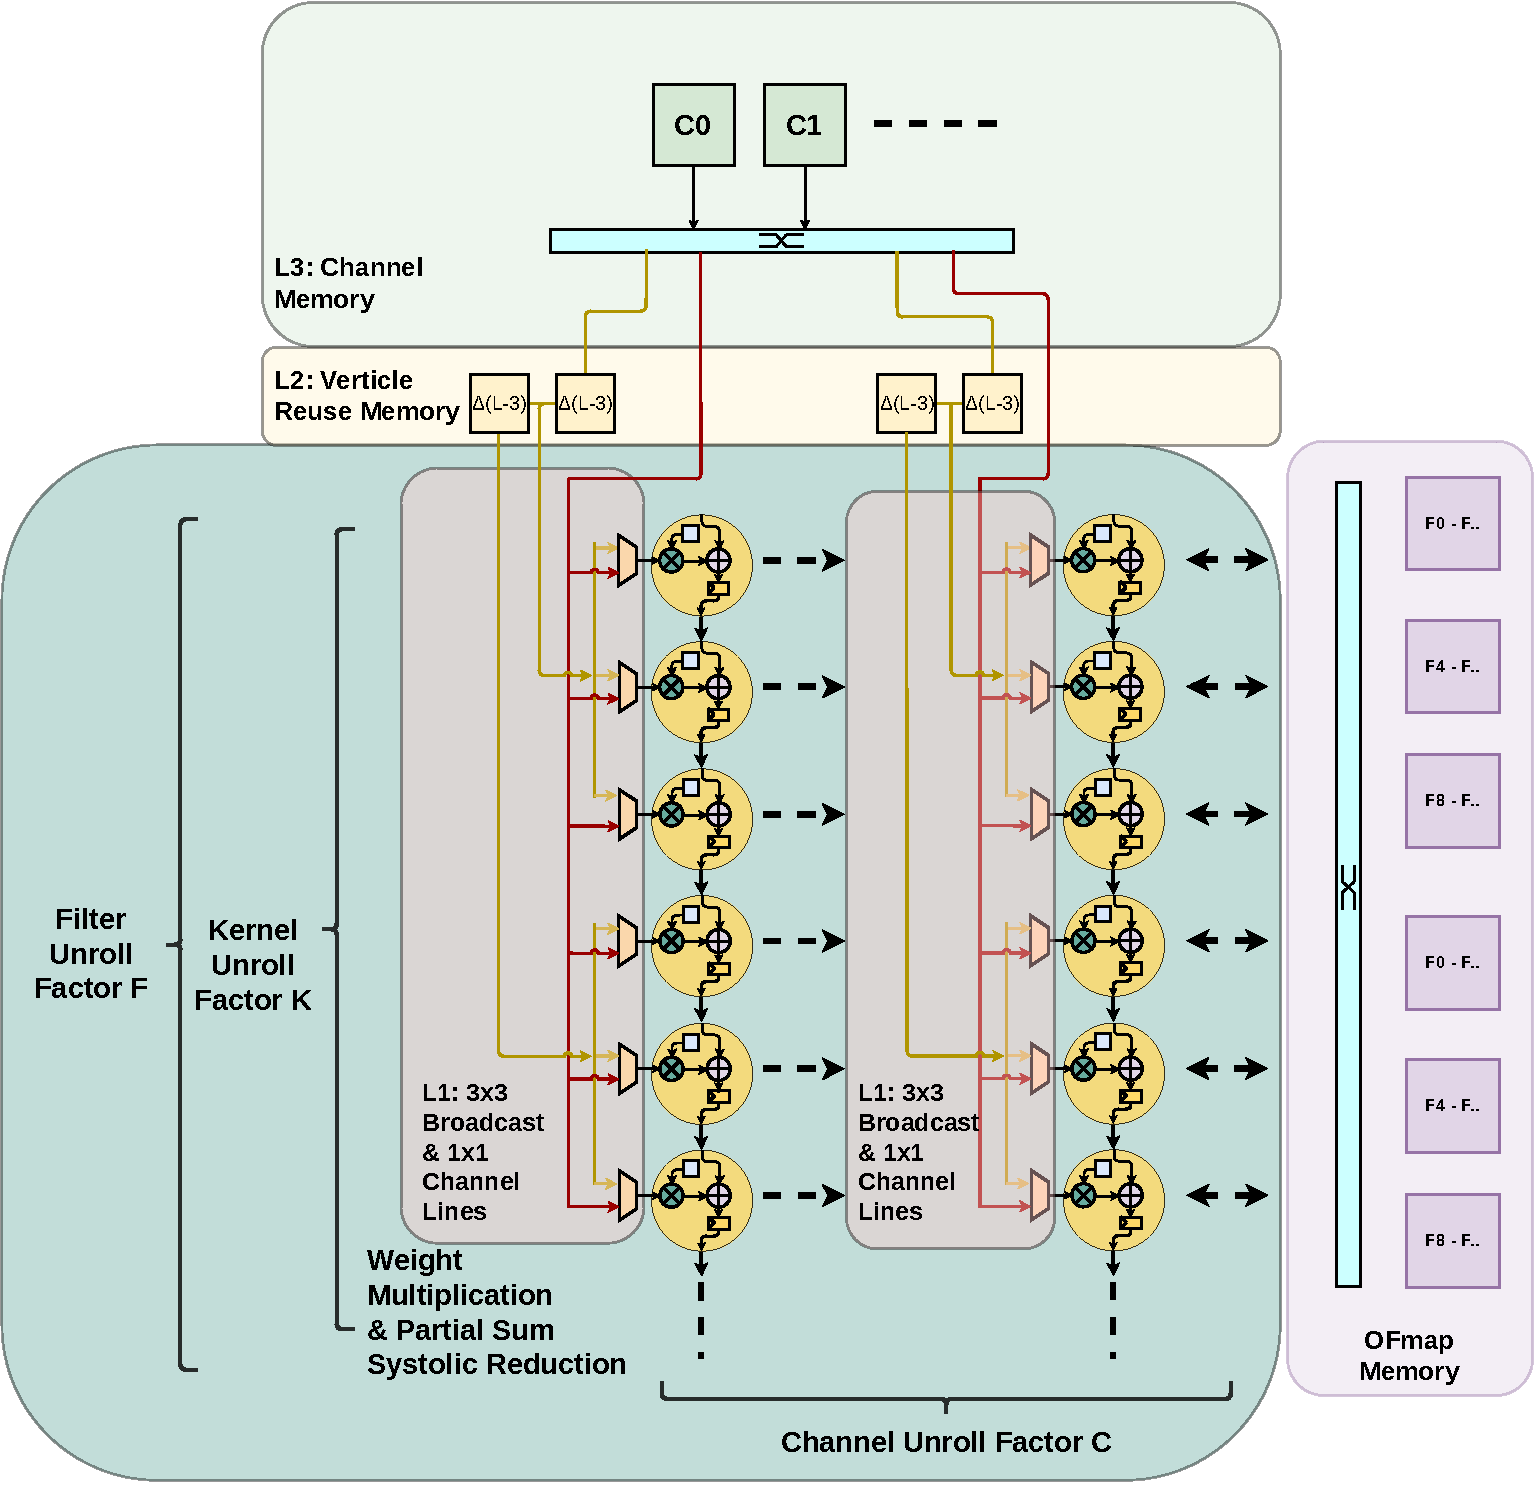
\includegraphics[scale=0.58]{fig/hero-t-verticle.pdf}
    \caption{HERO template with both Kernel and Filter loops mapped to the vertical axis}
    \label{fig:hero:vertical}
\end{figure}


